\documentclass[11pt,letterpaper]{article}
\usepackage[T1]{fontenc}
\usepackage{lmodern}
\usepackage[margin=1.15in]{geometry}
\usepackage{amsmath,amssymb,amsthm}
\usepackage{tikz}
\usepackage[hidelinks]{hyperref}
\hypersetup{pdftitle={VP and VNP are different},pdfauthor={OpenAI}}

\newtheorem{theorem}{Theorem}[section]
\newtheorem{corollary}[theorem]{Corollary}
\newtheorem{lemma}[theorem]{Lemma}
\newtheorem{proposition}[theorem]{Proposition}
\theoremstyle{definition}
\newtheorem{definition}[theorem]{Definition}
\numberwithin{equation}{section}
\DeclareMathOperator{\poly}{poly}
\DeclareMathOperator{\Res}{Res}
\DeclareMathOperator{\Tr}{Tr}
\setlength{\emergencystretch}{2em}
\setcounter{tocdepth}{1}

\title{VP and VNP are different}
\author{OpenAI}
\date{}

\begin{document}
\maketitle
\begin{abstract}
We prove that VP differs from VNP over every field. The lower bound holds for
border circuits and is superpolynomial, of the form $\exp(\Omega((\log n)^{5/4}))$. In particular
it applies to the permanent outside characteristic two. The proof trades two kinds of
hardness against one another: the rigidity of tensor networks priced in Euclidean space,
and the ability to diagonalize even against degenerating nonuniform circuits by replaying
their computations inside a wire budget.
\end{abstract}

\tableofcontents
\clearpage

\section{Introduction}\label{sec:introduction}

A polynomial can have an enormous number of terms and still be easy to compute. But
suppose that the only compression we know is the following one: the terms (with repetitions
allowed) can be described locally, or checked quickly given an index. Does this suffice?

Valiant's completeness theory \cite{Valiant,ValiantProjections} gave us a formal version of this question and
some of the most arresting concrete versions as well. $\mathrm{VP}$ over a field consists of families of
multivariate polynomials of polynomial degree in polynomially many variables, computable
by polynomial size arithmetic circuits; $\mathrm{VNP}$ allows, on top, summing over all settings of
polynomially many auxiliary inputs to zero and one. Here and throughout, size and degree
bounds for classes are polynomial in the family index, circuits are nonuniform, computing
with free field constants and binary additions, subtractions and multiplications, and the
computation is of formal polynomials. No assumptions are made about degrees along the
way. For background and formulations see e.g. \cite{BCS,Burgisser,BC2024,ShpilkaYehudayoff,BLMW}.

We give a negative answer. In fact we prove the geometric strengthening (cf. \cite{ApproxFactors}): $\mathrm{VNP}$
is not contained even in border $\mathrm{VP}$. By this we mean that we may take coefficient-wise
limits of circuits, in the sense of Zariski closure over the algebraic closure. To give the result
a quantitative form, take the family
\[
  f_n(Z) = \sum_{x\in\{0,1\}^n} c_x Z_{1,x_1}\cdots Z_{n,x_n}.
\]
Here $c_x$ counts accepting paths of an ordinary universal machine, running the program
encoded by a self-delimiting prefix of $x$, with $x$ itself as input. For definiteness permit
up to $n^{1000}$ bit steps per path (binary choices; reject malformed or over-clock paths);
any convenient efficient Turing machine conventions will do, with polynomial simulation
overheads comfortably inside that clock for the fixed programs used below.

\begin{theorem}[separation]\label{thm:separation}
Over every field, border circuits for $f_n$ require $\exp(\Omega((\log n)^{5/4}))$
gates. This is so even measuring approximation in degree $n$ only.
\end{theorem}

In particular, this concerns an integral family with particularly simple summands. The
$\mathrm{VNP}$ upper bound is standard: use auxiliary Boolean variables for $x$, branch choices (forcing
unused ones to zero), and an accepting Cook--Levin tableau \cite{Cook71,Levin} with unique auxiliaries.
The product of local indicator polynomials and $((1-x_i)Z_{i,0}+x_i Z_{i,1})_{1\le i\le n}$ (multiply these
factors also) is in $\mathrm{VP}$.

By the classical projection completeness theorems \cite{Valiant,ValiantProjections,Burgisser,BC2024}, we have:

\begin{corollary}\label{thm:projections}
The same lower bound in terms of matrix order holds for the directed
Hamiltonian cycle polynomial, and (except in characteristic two) the permanent. It holds
also for determinantal complexity (minimum order of a determinant of affine linear forms),
including border determinantal complexity. In particular for all sufficiently large $m$ and
\[
  m\le N\le \exp(c(\log m)^{5/4})
\]
with sufficiently small $c>0$, the degree-$N$ padded $m\times m$ permanent in characteristic zero is
excluded from the determinant orbit closure.
\end{corollary}

\begin{proof}
When only the degree in question is approximated, first homogenize to obtain exactly
that degree, at polynomial cost in the size and degree. Polynomial projections preserve
border upper bounds by continuity. Bounds at polynomially sampled dimensions give bounds
of this form at all large dimensions by standard padding (to force extra HC vertices subdivide
a vertex through a mandatory chain). Determinant has polynomial size over every field \cite{MahajanVinay}.
For orbit closure (affine cone, allowing extra ambient variables if needed), use that the orbit
consists of determinants of linear matrices and that padding by a power of a new variable
can be undone by specialization. Even padding by an existing variable works: split into
components by degree in that variable, discard too-low degrees and undo the shift, a linear
operation costing polynomial overhead.
\end{proof}

\paragraph{Where this sits.}
We mean separation at the polynomial scale; there are harder quasipolynomial questions (notice the
formulation already in \cite{Valiant}; see also \cite{MulmuleySohoni2008}), closely connected to
formula complexity by depth reduction \cite{Hyafil,VSBR}. Nor is this a separation for decision problems
in the Boolean model. But even the polynomial determinantal projection question by itself
has long been a benchmark open problem (e.g. \cite{AviICM}), and in orbit-closure form central to
geometric complexity theory \cite{MulmuleySohoni,MulmuleySohoni2008,BLMW,BIPnooccurrence}. We give
no explicit module of equations or
representation-theoretic obstruction; occurrence obstructions are known not to work for
standard GCT with large polynomial padding \cite{BIPnooccurrence}. Previous advances on determinantal
lower bounds include quadratic bounds \cite{MignonRessayre,CaiChenLi,LandsbergManivelRessayre} and,
in recent preprints, cubic border
bounds \cite{CubOAI,Sheshadri287} (see also the polar methods of \cite{SheshadriBorder2026} and
\cite{KumarVolk2026}). For unrestricted circuits think
of the $n\log d$ scale: gradient and degree give such lower bounds even on simple degree-$d$
polynomials in $n$ variables \cite{BaurStrassen,StrassenBezout}; see also the recent treatment and
permanent results in
\cite{TenAdvances}.

There is a magnificent history of large bounds after changing the problem slightly.
Monotonicity can force exponential bounds \cite{Val80,JerrumSnir}; symmetry too can come at a steep price
\cite{DawarWilsenach}. The multilinear world has superpolynomial bounds on formulas even for determinant
\cite{RazMultilinear}. Ranks of partial derivative matrices and relatives \cite{Nisan,NW97pd,CKW}
are ubiquitous; but
circuits give us low ranks across \emph{varying} cuts, which is quite different from a single matrix (cf.
the discrepancy and partition issues in \cite{Raz06,RSY08,AKV20,BFLY26,CKSS24}). There is the depth-four program
\cite{AgrawalVinay,Koiran2012,Tavenas2013} with formidable progress via shifted partials and beyond,
attaining even the
square-root scale in the exponent for homogeneous depth four, but with constants critical for
unrestricted circuit implications \cite{Kayal2012,GKKS14,KSS13regular,KLSS14,KumarSaraf2014}; see
\cite{DEP5OAI} for recent progress at depth five.
And there are now even superpolynomial bounds at arbitrary \emph{constant} depth
\cite{LSTconst,BDS24,Forbes2024}. For
more perspectives, including the power and possible limitations of proofs by low-complexity
equations, see \cite{ShpilkaYehudayoff,KSsurvey,Gro15,GKSS17,FSV18}. Here the approach will be
different, although varying cuts
play an essential role.

\paragraph{Strategy.}
Call a binary index in a tensor contraction a wire. Imagine placing the tensors in
Euclidean space, and charging length for each wire. We isolate a \emph{strict shortening} hypothesis.
Informally: is there some dimension and some fixed local tensor identity that communicates
along bundles of orthogonal diameters more cheaply than literally laying the wires? We can
allow alternatives (send a selector from the center to the terminals and sum).

\begin{itemize}
\item Without strict shortening, there is a direct, short proof. On a graph with independent
bundles along the edges, any balanced cut saving enough rank would allow wire to
be saved: reroute through a hub displaced a little in the direction of the resultant of
the cut wires. Even cuts chosen differently in different terms would work. This leads
quickly to Theorem~\ref{thm:separation}.
\item With strict shortening, we can save wire in computations. The point of saving is
to \emph{diagonalize}. Think of a coefficient of $f_n$ as a programmable processor. Against a
description of a circuit, compute this very coefficient, plus one. Now that sounds like
diagonalization against a linear bound at best. Instead take a contraction with very
many programmed processors in it; in its live execution it must be able to replay this
entire contraction with the hypothetical small circuit substituted for every processor.
It gets some important economies. First, the same circuit services all the queries: it
is possible to batch, charging essentially only degree per query since we compute by
counting and may follow just one parse tree. (For other kinds of batching see e.g.
\cite{Uhlig,Wbatch}.) And second, this computation can itself be performed as a contraction, with
RAM transcripts guessed and checked by sorting. So we can keep shortening its wires
so as to fit the processors' communication budget.
\item There are real difficulties with this program. Wire saving in big networks must be
made to \emph{iterate} (compare gap amplification in undirected network coding \cite{BGS}, though
here our alphabet may be contracted by summation and we even sum over wirings).
We build ribbon-like switching hosts: locally Euclidean along many axes, with vast
routing room; the cost accounting will pay even for concentration of traffic. We will
also need a final constant-factor squeeze, adapting the grid method of the recent \cite{Anthropic3SAT}
on counting SAT (cf. also \cite{Khoruzhii,ETHfalse}). And how can one learn, let alone distribute, a
circuit using arbitrary constants, possibly only working in a limit? We avoid that:
after collecting powers of all circuit parameters, insert certain universal weights. We
realize the limit as an eigenvector law for operators whose \emph{entries} can be replayed by
counting with very modest advice. Cartier operators in positive characteristic are key
to this step, even if we began in characteristic zero.
\end{itemize}

Thus the proof is not just a rigidity argument and not just an algorithmic lower bound
(for a different use of algorithms and diagonalization in lower bounds see \cite{Williams13}): if geometry
fails to prove hardness directly, its failure powers a hierarchy theorem. We organize the
proof around that hinge. After making shortening precise and giving the direct bound,
we state and reduce the contrasting \emph{stretch theorem} (\S\ref{sec:stretch})---stretch because a single fixed
saving will boost the lower bound to stretched exponential. Its reductions go to a boundary
lemma (\S\ref{sec:slicing}) and a replay lemma; the rest of the core argument constructs the replay. One
can also proceed directly to that construction (using the one-dimensional, exact version of
the boundary lemma for motivation), returning to \S\ref{sec:slicing} at the end.

\section{The hinge}\label{sec:hinge}

A bit tensor network has arbitrary local tables. Joining ports sums over a shared bit; multiply
all local entries and sum over assignments (external ports left as arguments). A width-$b$
cable joins $b$ pairs of ports. Place nodes in a metric space: charge width times distance for
each cable, including any run up to an external terminal. Thus local reblocking or other
computation at the same point costs nothing.

\begin{definition}\label{thm:shortening}
In dimension $D\ge 2$, let $C_{D,m}$ consist of width-$m$ cables on the $D$ coordinate
diameters of the Euclidean unit ball ($m\ge 1$). That is, the tensor at the $2D$ terminals testing
equality across all diameters. A strict shortening is a finite sum identity for this tensor over
a field, using $A$ networks in the ball each of cost $\le w$ where
\[
  w + 2D\log_2 A < 2Dm.
\]
\end{definition}

We take log base two throughout. We can equally well begin with membership in
the closure of such sums (fixed finite layouts, variable tables, algebraically closed field).
Indeed the $t$-th tensor power lies in the span of $t$-th powers of actual sums since this span
is closed. It requires only polynomially many (in $t$, by counting monomials in the fixed
ambient dimension). Thus at width $tm$ we get an exact sum with $\poly(t)A^t$ terms of cost
$\le tw$. Taking powers we can and will even pay for rounding up the log. Positions can be
made rational; the saving is strict. Also existence in any characteristic is unchanged among
algebraically closed fields there, by the Nullstellensatz.

Here is how we actually use one. For $j$ juxtaposed crossings, sum over profiles $(j_1,\ldots,j_A)$
of multiplicities, one layout for each. \emph{Within} a layout, send a word of $j$ selectors (constrained
to have that profile) from the origin to all terminals; sum on it. Copies of each term operate
on assigned terminal blocks in order of occurrence; inner nodes can use separate cables per
term, with widths proportional to $j_a$, not needing to see the selectors. This realizes the
tensor exactly, each layout saving a fixed fraction of length, and with a bounded number
of cable descriptions (widths $O(j)$). Local operations are word parsing, reblocking, and
applying constant tables.

\subsection{If wire cannot be saved}

Suppose no strict shortening works (any $D,m$) over an algebraically closed field. Take a
bounded-degree expander on $d\asymp a\sqrt{\log n}$ vertices, so every balanced cut (sides of size at
least $d/3$) has at least $\gamma d$ edges across it. Here $\gamma >0$ is absolute, $a>0$ a small constant to
choose (for expanders see \cite{HLW}). Use bundles of $m=\lfloor c\log n\rfloor$ bits ($c>0$ sufficiently small) on
each edge, and a variable for each vertex and setting of its incident bits. The polynomial $g$ is
the partition function: multiply one variable per vertex and sum over consistent assignments.
With the variables as slots grouped by vertex, its coefficient tensor consists simply of wires
(for context on graph contractions see e.g. \cite{MarkovShi}).

This is an ordinary projection of $f_n$: the bits $x$ include one-hot choices of vertex variables,
checked for consistency by the deterministic program in a forced prefix (also including graph
data, rejecting nonzero padding). Insert each variable for the corresponding ``one'' weight;
there is room since the number of variables is at most $n^{1/2}$ with $c$ small. If $f_n$ has border
cost $s$ as in Theorem~\ref{thm:separation}, then (first homogenizing) $g$ has full border cost $\poly(n+s)$.

Consequently its coefficient tensor is in the closure of sums with one term per balanced
cut, of rank across that cut bounded by
\[
  2^{O(d)}\poly(n+s).
\]
Indeed apply the usual balanced-product decomposition to the set-multilinear component of
actual circuit outputs. Keep components multilinear in distinct variable \emph{groups} (multidegrees
zero or one) throughout with $3^{O(d)}$ overhead. In the output expansion collect uses of a first
balanced gate (group set of balanced size), descending from the output in a parse tree through
linear choices and through the larger child at products (fix ties); one is necessarily reached.
Terms at each such gate factor into its polynomial times a polynomial on complementary
groups. See e.g. \cite{ValiantProjections,VSBR,Raz13rank} for related cuts and multilinearization.

Place the graph tensor as $C_{D,m}$, one diameter per edge ($D=O(d)$), taking the independent
terminals out of their vertex groups. For a term, stream all bits in to two hubs (one
per side). Factor there with a bridge of at most
\[
  h=C(d+\log(n+s))
\]
bits by the rank bound. With hubs at zero this just matches the direct cost. But the unit
position vectors of the terminals served by the first hub have a sum of norm at least $\sqrt{\gamma d}$.
Move that hub in the direction of this sum by $u=b/\sqrt{d}$. Using $\sqrt{1+x}\le 1+x/2$, change
of cost is at most
\[
  -mu\sqrt{\gamma d} + Dmu^2+ hu.
\]
With $b>0$ fixed small and $h\le m\sqrt{\gamma d}/2$, this saves a constant times $m$. Paying at most
$2Dd$ for selection still gives a strict saving if $a$ is small enough. Hence $h$ must be larger.
This proves Theorem~\ref{thm:separation} in the indicated case.

\section{Stretch theorem and reduction}\label{sec:stretch}

Here is what we have left to prove.

\begin{theorem}[stretch]\label{thm:stretch}
If a strict shortening exists in the characteristic over consideration
(which may be zero), then the border cost in Theorem~\ref{thm:separation} exceeds $2^{n^\sigma}$,
some $\sigma >0$, for all
sufficiently large $n$.
\end{theorem}

We use the integral universal parse map for circuits of size $M$, into the space of \emph{all}
coefficients of homogeneous degree $n$ in the $2n$ variables. Here is one version. Use a
$\poly(n,M)$ palette of gates per positive degree $\le n$. Each leaf gate is a linear combination
of variables with new parameters; each higher gate is the sum of all ordered products of two
gates of smaller degrees adding correctly, each product weighted by a new parameter. Use
one designated final gate. With large enough palettes this covers the degree-$n$ component
of every circuit of size $M$: form positive homogeneous components (degree-zero ones are
scalars), absorbing linear combinations. Let $Y(X)$ be the map, $X=(X_1,\ldots,X_h)$ the
parameters. Output coordinates have parameter degree $2n-1$ (one choice per node of an
ordered parse tree, $n$ leaves). Parameter indices can use a regular format, e.g. complete
tuples padded with unused parameters.

Fix exact shortening data, reducing its constants into a finite field when needed; for
characteristic zero one presentation over a number field works outside a fixed finite set of
primes. We take all fixed exponents in resource constructions rational where appropriate.
For a sufficiently small fixed $\rho >0$ (depends on shortening data), put
\[
  \sigma=\rho/2,\qquad M=2^{\lceil n^\sigma\rceil},\qquad r=2^{\lceil n^\rho\rceil},\qquad L=r^2.
\]
Write $c$ for the full coefficient vector ($0$ on slots outside the pattern).

\begin{lemma}[replay]\label{thm:replay}
Work modulo a prime $p$ with $\poly(M)$ bits, with the exact shortening,
over a finite extension with arithmetic (including field presentations and shortening coefficients)
of bit complexity $\poly(M)$. Take square matrices $W_\mu$ over the prime field on binary
indices (called pins), with pin length $\poly(M)$, one matrix per parameter monomial $X^\mu$ of
degree $\le L$. Entries indexed by monomial and two pins are available by counting modulo
$p$ with $\poly(M)$ cost per path and $\poly(M)$ bits of advice. Mark any one pin $\ast$. Then, for
all sufficiently large $n$, there is a row vector of polynomials $F$ over the prime field of degree
$\le L/(2n)$ in coefficient slots, with
\[
  F(c) = e_\ast+ \sum_\mu \bigl([X^\mu] F(Y(X))\bigr) W_\mu,
\]
where $e_\ast$ is the row unit vector.
\end{lemma}

As usual these asymptotic assertions work also on unbounded sets of $n$, with fixed
polynomial bounds and primes allowed to vary.

\begin{lemma}[boundary evaluation]\label{thm:boundary}
Suppose $c$ belongs to the degree-$n$ border image (closure
of the parse map image) in fixed characteristic. Use that prime in positive characteristic; in
characteristic zero we can take a prime as in Lemma~\ref{thm:replay}, avoiding any fixed finite list. There
exist matrices as in that lemma, and a nonzero column $\Omega$ over the prime field, such that
\[
  \left(\sum_\mu[X^\mu](G(Y(X))) W_\mu\right)\Omega=G(c)\Omega
\]
for every prime-field polynomial $G$ in coefficient slots of degree $\le L/(2n)$.
\end{lemma}

If we had $c=Y(a)$ in a small prime field, we could simply take scalar weights $a^\mu$. Matrix
weights will let us stay local even at a boundary point reached with high-degree constants
and large poles.

\begin{proof}[Proof of Theorem~\ref{thm:stretch} from the lemmas]
If a border circuit exists along an unbounded sequence, apply Lemma~\ref{thm:boundary}, then
Lemma~\ref{thm:replay} marking a nonzero position of $\Omega$. Multiply the
replay equation by $\Omega$ and cancel using the boundary equations: $e_\ast \Omega=0$, a contradiction.
\end{proof}

\section{Evaluation on the boundary: slicing to a curve}\label{sec:slicing}

We prove Lemma~\ref{thm:boundary}, in this and the next section. Measure polynomial and singly exponential
($2^{\poly(M)}$) in $M$. Write $T_X(Z)=\sum_\nu Y_\nu(X)Z^\nu$ for the parse map output, reindexing $Z$ from
$1$ to $2n$, and $d=2n-1$; remember that $Y$ has degree $d$ and its coordinate polynomials have
coefficient $\ell^1$ norms with polynomial bit length, by counting parses.

\subsection{A prime of modest size}

We recall three geometric degree bounds, using the degree of the projective closure in the
affine case (see \cite[Ch. I, \S7]{Hartshorne} and \cite[Lemma 2 and Proposition 3]{Heintz}). A linear image of an
irreducible variety has closure of degree at most the degree of the variety. More generally,
the closure of an image of an open subset of $\mathbb{A}^h$ under a rational map with a common
denominator and all degrees at most $e\ge 1$ has degree at most $e^h$. Indeed a general linear
section of complementary dimension meets the image closure in its attained locus in as many
distinct points as its degree. The pullbacks must have at least one component per such
point. Bézout bounds this number, including when a pullback intersection has components
of several dimensions: in a cut of degree at most $e$ the sum of $(\deg V)e^{\dim V}$ over components
cannot increase. In particular, successive linear sections never increase the total degree.

Finally, if a point is outside an irreducible closed set of degree $D$ and dimension $b$, an
equation of degree at most $D$ separates them. Indeed, project the projective closure to $\mathbb{P}^{b+1}$
from a linear center disjoint from its join with the point. The image is a hypersurface (a
positive-dimensional projective fiber would meet the center), and misses the projected point.
Its equation pulls back to one as asserted. In codimension one use the hypersurface equation
itself. These arguments work over any algebraically closed field. For a reducible set one can
multiply the separating equations of its components.

\begin{lemma}\label{thm:reduction}
If $c\in\overline{Y(\mathbb{A}^h)}$ over $\overline{\mathbb{Q}}$, there is a prime $p$ of polynomial
bit length for which
the same inclusion holds over $\overline{\mathbb{F}}_p$. The fixed tensor identities can be specialized at the same
prime, with coefficients of bounded extension degree.
\end{lemma}

\begin{proof}
In every characteristic the closure has degree at most $D=d^h$. Form the integer
matrix whose column for a monomial $y^\eta$, $|\eta|\le D$, is the coefficient vector of $Y(X)^\eta$ in
the $X$-monomials of degree at most $dD$. Let $u=(c^\eta)_{|\eta|\le D}$. By the closure hypothesis $u$
annihilates the rational kernel and hence is in the rational row span. The number of columns
can be very large, but the number of rows is only $\binom{h+dD}{h}$
, a single exponential. Every entry
has at most singly exponential bit length by submultiplicativity of the coefficient norm.
Choose a basis of rows and a square nonsingular minor on those rows. Cramer's rule on its
columns gives a row expression for $u$ with common denominator dividing the determinant.
The expression holds on all columns because $u$ is in the row span. Hadamard's inequality
bounds the bit length of the determinant by a single exponential.

The fixed constants lie in a number field and are integral after inverting a fixed integer.
Outside its prime divisors we may reduce at any prime ideal above $p$, obtaining a residue
field of degree at most the number-field degree. All tensor identities survive, as do any
fixed nonvanishings after excluding finitely many more primes. The prime number theorem
supplies a prime $p$ of polynomial bit length outside these exclusions and coprime to the
determinant: the logarithm of the product of primes up to $x$ grows linearly in $x$. The
reduced row expression now shows, even after scalar extension, that every relation of degree
$\le D$ on the reduced image vanishes at the reduced $c$. The separating-equation bound proves
the inclusion.
\end{proof}

Henceforth write $\mathcal{K}=\overline{\mathbb{F}}_p$. In fixed positive characteristic we keep the
original prime. In
characteristic zero the chosen $p$ may depend on $n$. In either case let $E_0$ be a finite field
containing the constants for the fixed identities. Its degree over $\mathbb{F}_p$ is bounded independently
of $n$.

\subsection{Equations for the branch}

Lehmkuhl and Lickteig for tensors, and Bürgisser for circuits, used the degree of a graph
to bound the cost of passage to a limit \cite{LehmkuhlLickteig,ApproxFactors}. Guo, Saxena and Sinhababu obtained
bounded-degree approximations for approximate polynomial satisfiability over arbitrary
fields \cite[Theorem 4.2]{GSS}. Here the parameter on the curve must also be separable, and each
defining equation must admit a short evaluator.

\begin{proposition}\label{thm:branch}
There are a finite extension $E$ of $E_0$, with $\log_2|E|$ polynomial, and $h$
polynomials $g_i(X,t)\in E[X,t]$ of polynomial degree with the following properties. Their
common zero set over $\mathcal{K}$ has an irreducible curve component of singly exponential degree,
dominant over the $t$-line, on which $J=\det(\partial g_i/\partial X_j)$ is generically nonzero. The function
field of this curve has a place above $t=0$ at which all $Y_\nu$ are regular with residue $c_\nu$. With
polynomial advice, each $g_i$ can be evaluated in polynomial bit time over $E$ or a specified
extension of polynomial bit length, given its field representation and the embedding of $E$.
\end{proposition}

\begin{proof}
Close the graph of $Y$ in $\mathbb{P}^h \times \mathbb{A}^{\{\nu :|\nu|=n\}}$, using homogeneous
parameter coordinates
$(1:X)$. Projection to the output space is closed, so the fiber over $c$ is a nonempty projective
set. On each of the $h+1$ standard parameter charts the graph closure has degree at most
$(d+1)^h$. In fact, on its dense affine-parameter part it is parametrized by $(X,Y(X))$ with
the parameter coordinates expressed as ratios having a common linear denominator. After
multiplying each output polynomial by this denominator, all numerator degrees are at most
$d+1$. The fiber in each chart is a linear section, so the total number and sum of degrees of
its projective components are at most $(h+1)(d+1)^h$, by counting every component in a
chart that meets it.

We first isolate a point of the fiber, allowing it to lie at parameter infinity. Cut the
projective fiber by hyperplanes in the parameter coordinates until it is finite. At each
cut choose a hyperplane containing none of the positive-dimensional components. Every
top-dimensional component meets it by projectivity, so the final cut retains a point. The
number of forbidden linear conditions on the hyperplane coefficients is at most the degree
bound above. Fix one retained geometric point $P$ and choose a standard chart containing it.
Write $z=(z_1,\ldots,z_h)$ for its coordinates, $y$ for the output coordinates, $G$ for the chart of
the graph closure, and $\ell_1(z),\ldots,\ell_b(z)$ for the hyperplanes just used in this chart. In $G$, the
common zeros of the $y_\nu-c_\nu$ and the $\ell_j$ now form a finite nonempty set.

We choose $h$ linear combinations of these equations that still have finitely many common
zeros and can be evaluated without listing the output coordinates. Put $B=(n+1)^{2n}$ and
$e(\nu)=\sum_{j=1}^{2n}\nu_j(n+1)^{j-1}$. For a scalar $a$ use the form
\[
  D_a(z,y) = \sum_\nu a^{e(\nu)}(y_\nu-c_\nu) + \sum_{j=1}^b a^{B+j}\ell_j(z).
\]
All exponents are distinct. On any positive-dimensional component of the current intersection
some original equation is nonzero at some point. At that point $D_a$ is a nonzero polynomial
in $a$ of degree at most $B+b$. Choosing $a$ outside its roots for each component cuts their
dimensions by one. The number of components stays bounded by $\deg G$ under linear sections.
After $h$ choices we have forms $D_1,\ldots,D_h$, now indexed by the order of selection. Their
common zero set in $G$ is finite and contains $P$.

We next make the generic fiber separable. The deformation must pass through $P$ when
$t=0$, even if every output derivative vanishes. We can thus add a linear term multiplied by
$t$ to each equation. Write $D=(D_1,\ldots,D_h)$ and use the equations
\begin{equation}\label{eq:deformation}
  D_i(z,y)+t(z_i-v_i)=0 \qquad(1\le i\le h).
\end{equation}
Over $\overline{\mathcal{K}(t)}$ these describe a fiber of the affine linear map
$\psi_t(z,y)=z+t^{-1}D(z,y)$. Let $U\subset G$
be the locus of finite parameters. It is an open subset of affine $z$-space, with $y=Y(X(z))$.
Write $\widetilde{D}(z)=D(z,Y(X(z)))$. The determinant $\det(tI+\partial \widetilde{D}/\partial z)$
on $U$ is monic in $t$ over
$\mathcal{K}(G)$. In particular its zero set on $U$ over the generic $t$ has dimension less than $h$. The
same is true of $G\setminus U$. Their image closures under $\psi_t$ therefore lie in a proper hypersurface
of singly exponential degree. For the degree estimate, $G\setminus U$ is cut out by the vanishing
of one chart coordinate (or is empty). On $U$ the $X$ are ratios of affine linear forms with
a common denominator, so each $D_i(z,Y(X(z)))$ has such a denominator to power $d$ and
numerator degree at most $d+1$. Clearing the derivatives' denominators in the determinant
gives a polynomial of degree $O(h(d+1))$ in $z$. Intersect $G$ with this polynomial and apply
the linear-image and separating-equation bounds above. Choose $v$ outside the resulting
hypersurface. Every point of the generic fiber then has finite parameters and invertible
$z$-Jacobian.

The hyperplane coefficients, the scalars defining $D_1,\ldots,D_h$, and the vector $v$ can all
be chosen in one extension $E$ of $E_0$ of singly exponential cardinality. Indeed, all excluded
sets were zeros of nonzero polynomials of singly exponential total degree, uniformly in the
previous choices. A grid of larger side length avoids each such polynomial, including one
with coefficients in $\overline{\mathcal{K}(t)}$. Finite extensions of $E_0$ with this size bound
exist since $\log_2|E_0|$ is
polynomial.

At $(P,0)$, Krull's dimension theorem gives local dimension at least one for the $h$ equations
in \eqref{eq:deformation} in $G\times \mathbb{A}^1$. The special fiber is finite and the generic
fiber has dimension at most
zero by the Jacobian calculation. Thus there is a curve through the point dominant over
the $t$-line. A point above it on the normalization gives the claimed place: every output
coordinate $y_\nu$ is regular there and equals $c_\nu$ at the point. The parameter functions $X_j$
themselves can have poles there.

To obtain equations in the original circuit parameters, let $\delta(X)$ be the chart denominator
and write $z_i=u_i(X)/\delta(X)$ with $u_i,\delta$ affine linear. Then
\[
  g_i(X,t) = \delta(X)D_i\bigl(z,Y(X)\bigr) + t\bigl(u_i(X)-v_i\delta(X)\bigr)
\]
is a polynomial since $D_i$ is affine linear in $z,y$. On $U$, multiplication by $\delta$ scales each Jacobian
row by a unit at a zero, and the change between $z$ and $X$ has invertible Jacobian. The
affine closure of the resulting curve in $X,t$ is therefore a component with $J\ne 0$ generically.
Its degree is at most $(d+2)^h$ by Bézout, since each $g_i$ has total degree at most $d+2$. In
particular $dt$ spans its function-field differentials over $\mathcal{K}$: the $dg_i=0$ express every $dX_j$ as a
multiple of $dt$, and this space has dimension one since $\mathcal{K}$ is perfect.

Finally, the weighted sum of output coordinates in $D_a$ is evaluated by one evaluation of
the original homogeneous table,
\[
  \sum_\nu a^{e(\nu)}Y_\nu(X) = T_X\bigl(a^{(n+1)^0},\ldots,a^{(n+1)^{2n-1}}\bigr).
\]
The single offset $\sum_\nu a^{e(\nu)}c_\nu$ for each chosen $a$ is advice. The circuit for the homogeneous
table is specified by its slot and degree ranges from our parse map; its weights are the input
variables $X$. The slice coefficients, $v$, offsets and finite-field arithmetic data together use
polynomially many advice bits. All exponents in this evaluation have polynomial bit length.
Repeated squaring and the homogeneous table recursion therefore evaluate the numerator
polynomial $g_i$ in polynomial bit time, including at inputs where the chart denominator is
zero. The field $E$ contains the coefficients of the equations and offsets. The point $P$ and
the chosen branch can be defined over larger fields because the evaluator uses only these
equations and offsets.
\end{proof}

\section{Reading a boundary value with residues}\label{sec:residues}

Let $g_1,\ldots,g_h \in E[X_1,\ldots,X_h,t]$ be the equations from Proposition~\ref{thm:branch}, and fix its branch
over $t=0$. The parameters $X_i$ may have poles there, even though all the outputs $Y(X)$
are regular with value $c$. A computation path sees only one monomial. Regularity at the
chosen place can come from cancellation between distinct paths. We assign each weighted
monomial a matrix with entries given by short counting paths. After summing the matrices,
one fixed nonzero vector recovers the value of every regular sum whose residue belongs to
the prime field. Throughout this section, polynomial and single-exponential bounds are in
the parameter $M$ of Section~\ref{sec:slicing}.

\begin{lemma}[Residue pins]\label{thm:pins}
Fix a single-exponential degree bound $L$. There are a nonzero
vector $\Omega\in\mathbb{F}_p^d$ and $d\times d$ matrices $W_{a,\mu}$ over $\mathbb{F}_p$, indexed
by $a\in E$ and $\mu\in\mathbb{Z}_{\ge 0}^h$ with $|\mu|\le L$,
with the following property. If $A=\sum_\mu a_\mu X^\mu \in E[X]$ has degree at most $L$, is regular at the
branch and has value $z\in \mathbb{F}_p$, then
\begin{equation}\label{eq:eigenvector}
  \biggl(\sum_\mu W_{a_\mu,\mu}\biggr)\Omega=z\Omega.
\end{equation}
In particular this holds for $A=F(Y(X))$ of degree at most $L$, with $F$ over $\mathbb{F}_p$ and $z=F(c)$.
The matrices depend $\mathbb{F}_p$-linearly on $a$. Their dimension $d$ is single exponential. With one
polynomial-length advice string for all $a,\mu$ and all index pairs, any specified entry is the sum
modulo $p$ of the outputs of polynomial-time binary-guess paths returning $0$ or $1$.
\end{lemma}

Taking $W_\mu=W_{1,\mu}$ gives Lemma~\ref{thm:boundary}.

The proof uses test differentials $\eta$ on the curve. If $A$ has value $z\in \mathbb{F}_p$, then $A^q-z$
vanishes to order at least $q$ for every $p$-power $q$. Once $q$ exceeds the pole order of $\eta$, the
differentials $A^q \eta$ and $z\eta$ have equal residues. The Cartier identity $C_q(A^q \eta)=AC_q(\eta)$ moves
the power from the unknown function to an operation on the given test. We choose finitely
many tests for which the coefficients of $AC_q(\eta)$ can be read one monomial at a time. This use
of finite-dimensional actions on differentials is related to the Cartier transitions in Bridy's
work on automatic sequences \cite{Bridy}.

\subsection{Cartier extraction in the parameter coordinates}

Write $x=(x_1,\ldots,x_h)$ for the coordinate functions on the chosen geometric curve and
$K=E(t,x)$ for the subfield they generate. The extension $K/E(t)$ is finite: each $x_i$ is
algebraic over $\overline{\mathbb{F}}_p(t)$ and only finitely many algebraic constants occur in an equation for it.
Restrict the branch valuation to $K$ and normalize it to have value group $\mathbb{Z}$. Its residue
field $\kappa$ is finite, since this place lies over $t=0$ in a finite function field extension. The
functions $Y(x)$ still have residue $c$. For a uniformizer $s\in K$, the completion is $\kappa((s))$, with
the coefficient field obtained by lifting the roots of $T^{|\kappa|}-T$. Put
\[
  J = \det\left(\frac{\partial g_i}{\partial X_j}\right), \qquad \eta_0= \frac{dt}{J(x,t)}.
\]
The Jacobian is nonzero at the generic point. Differentiating $g_i(x,t)=0$ therefore expresses
all $dx_j$ as multiples of $dt$. This also proves $dt\ne 0$ in the completion. Indeed, $s\in E(t,x)$, so
$ds$ is a multiple of $dt$, while $s$ is the local uniformizer and $ds\ne 0$. This argument allows
ramification at $t=0$.

Put $Z=(X_1,\ldots,X_h,t)$. For each $q=p^u$ with $u\ge 1$, define the following operator on
Laurent polynomials:
\[
  \Lambda_q\left(\sum_j v_j Z^j\right) = \sum_i v_{qi+(q-1)\mathbf{1}}^{1/q} Z^i.
\]
On differentials in $\kappa((s))$, use the one-variable version
$C_q(\sum_j v_j s^j\,ds)=\sum_i v_{qi+q-1}^{1/q}s^i\,ds$.
Thus $C_q(D^q \eta)=DC_q(\eta)$ and $\Res(C_q \eta)=(\Res\eta)^{1/q}$, where $\Res$ extracts the coefficient of
$s^{-1}ds$.

\begin{lemma}\label{thm:cartier}
For $f\in E[X_1,\ldots,X_h,t,t^{-1}]$ one has
\begin{equation}\label{eq:cartier}
  C_q\bigl(f(x,t)\eta_0\bigr) = \Lambda_q\left(f\prod_{i=1}^h g_i^{q-1}\right)(x,t)\,\eta_0.
\end{equation}
\end{lemma}

\begin{proof}
We give the change of coordinates, which recovers the plane-curve formula of Stöhr
and Voloch when $h=1$ \cite[Theorem 1.1]{StoehrVoloch}. In characteristic $p$, Cartier on top differentials
commutes with the field embedding used below \cite{Cartier,Katz}. Recall the reason. In coordinates
$z_1,\ldots,z_b$ forming a $p$-basis, every coefficient expands uniquely in $z^j$, $0\le j_i<p$, over the
subfield of $p$-th powers. Modulo exact top forms, only the term with all $j_i=p-1$ survives:
all others have an antiderivative in some coordinate, and an exact form has zero coefficient in
that position. The inverse Cartier isomorphism from top forms to this quotient is intrinsic,
given on decomposable forms by
\[
  a\,dv_1\wedge\cdots\wedge dv_b \longmapsto \left[a^p\bigwedge_{i=1}^b v_i^{p-1}dv_i\right].
\]
Indeed, $v^{p-1}dv$ is closed, obeys the product rule with scalars raised to the $p$-th power, and is
additive modulo exact forms. For additivity the correction is the differential of the reduction
of the integral polynomial $((U+V)^p-U^p-V^p)/p$. These identities give naturality, and the
$p$-basis calculation gives the inverse. Iterating gives the stated coefficient rule for $q$. In an
iterated Laurent series field over a perfect field the successive series variables form a $p$-basis,
by grouping exponents modulo $p$.

Work over $\kappa((s))$ and introduce independent formal variables $y_1,\ldots,y_h$. Since
$J(x,t)$ is invertible in this coefficient field, the formal implicit function theorem gives
$\widetilde{x}\in \kappa((s))[[y_1,\ldots,y_h]]^h$ with $\widetilde{x}(0)=x$ and
$g_i(\widetilde{x},t)=y_i$. Substitution $X\mapsto\widetilde{x}$, $t\mapsto t(s)$
embeds the ambient rational function field into the corresponding iterated Laurent series field:
its image contains the algebraically independent $t(s),y_1,\ldots,y_h$. Under this substitution,
\[
  dX_1\wedge\cdots\wedge dX_h\wedge dt = J(\widetilde{x},t)^{-1}\,dy_1\wedge\cdots\wedge dy_h\wedge dt.
\]
Multiply by $f\prod_i g_i^{q-1}$ and apply Cartier in the two coordinate systems. In the ambient
coordinates its coefficient becomes $\Lambda_q(f\prod_i g_i^{q-1})$. In the series coordinates the
factor $\prod_i y_i^{q-1}$
ensures that the constant $y$-coefficient after Cartier comes solely from the constant term
of $f(\widetilde{x},t)/J(\widetilde{x},t)$ before Cartier. Equating the two constant coefficients,
with $dt=t'(s)\,ds$,
proves \eqref{eq:cartier}.
\end{proof}

\subsection{A finite family of tests}

Write $S=\sum_i \deg g_i$ and take $H=4(L+S+2)$. Use the box
\[
  \mathcal{B}=\{X^\alpha t^j: 0\le\alpha_i\le H,\ -H\le j\le H\}.
\]
For $f\in \mathcal{B}$ the Laurent polynomial
\begin{equation}\label{eq:test}
  aX^\mu\Lambda_q\left(bf\prod_i g_i^{q-1}\right),\qquad a,b\in E,\quad|\mu|\le L,
\end{equation}
is supported in $\mathcal{B}$. Indeed, raising $\prod_i g_i$ to the power $q-1$ increases each upper exponent
by at most $(q-1)S$. Extraction divides its upper bound by $q$, and multiplication by $X^\mu$
adds at most $L$. The resulting upper bound $H/q+S+L$ is at most $H$. The extracted $X$
exponents stay nonnegative and the lower $t$ exponent is at least $-H/q-1$.

The pole orders of the box differentials $f(x,t)\eta_0$ at our place are at most single exponential.
To see this, work first on the normalized projective model of the geometric curve of degree
$D$. A quotient of polynomials of degrees at most $e$ whose denominator does not vanish
identically on the curve has pole orders at most $eD$. Indeed, homogenize to the same degree
and intersect the curve with the denominator hypersurface. Bézout gives $D\le \prod_i \deg g_i$, a
single exponential by Proposition~\ref{thm:branch}. For $f/J$ one can take $e=(h+2)H+S$, clearing
negative powers of $t$. Restricting the valuation to $K$ and normalizing can only decrease these
pole orders. Finally $dt$ is regular at the place, since $t$ has positive valuation. Take $q$ to be
the first positive power of $|E|$ exceeding the bound. It is still single exponential.

Let $\ell(\eta)=\Tr_{\kappa/\mathbb{F}_p}(\Res\eta)$. Absolute trace is invariant under inverse Frobenius, so
$\ell(C_q \eta)=\ell(\eta)$. Index the pin vector by an $\mathbb{F}_p$-basis element $b$ of $E$ and
a box monomial $f$,
setting
\[
  \Omega(b,f)=\ell(bf(x,t)\eta_0).
\]
These entries belong to the prime field. At least one is nonzero. Indeed, the finite separable
extension $\kappa/\mathbb{F}_p$ has surjective trace. Lift a trace-one element of $\kappa$ to a function $w$ in the
valuation ring of $K$. Then $\ell(w\,ds/s)=1$. Express $(w\,ds/s)/\eta_0\in K$ as a finite linear
combination of $x$-monomials over $E(t)$, using the finiteness of $K/E(t)$ and the fact that $x$
generates it. Approximate each rational coefficient by a Laurent polynomial in $t$ over $E$. The
approximations preserve the residue if taken sufficiently far, since $t$ has positive valuation.
Thus some polynomial $f_0 \in E[X,t,t^{-1}]$ has $\ell(f_0(x,t)\eta_0)=1$. Apply Lemma~\ref{thm:cartier} with an
arbitrarily large $p$-power $Q$. The Laurent polynomial $\Lambda_Q(f_0 \prod_i g_i^{Q-1})$ is
supported in $\mathcal{B}$ once
$Q$ exceeds the absolute values of all exponents of $f_0$: extraction divides these exponents by
$Q$ and adds at most $S$. Its traced residue against $\eta_0$ is still one. Expanding its coefficients
in the basis proves the assertion. Only the existence of a nonzero index uses $Q$ or $w$. The
matrices will use the smaller power $q$ fixed by the pole bound.

\begin{proof}[Proof of Lemma~\ref{thm:pins}]
In row $(b,f)$ of $W_{a,\mu}$ put the prime-field coefficients of \eqref{eq:test} in their
respective columns $(b',f')$. The scalar $a$ multiplies the extracted polynomial, so the row is
$\mathbb{F}_p$-linear in $a$. By Lemma~\ref{thm:cartier}, the $(b,f)$ entry of the left side of
\eqref{eq:eigenvector} is
\[
  \ell(A\,C_q(bf\eta_0))=\ell(C_q(A^q bf\eta_0))=\ell(A^q bf\eta_0)=z\,\ell(bf\eta_0).
\]
Here the curve evaluations are understood. The final equality uses $A^q-z=(A-z)^q$, whose
zero of order at least $q$ cancels every pole of the test differential. This proves the eigenvector
identity for the entire regular sum. For a boundary value $z\in E$ the same computation gives
$R_z \Omega$, since $z^q=z$. Here row $(b,f)$ of $R_z$ expands $zb$ in the basis while keeping $f$ fixed.

It remains to compute an entry with short paths. The index set has size
$[E:\mathbb{F}_p](H+1)^h(2H+1)$, so indices have polynomial bit length. For a prescribed column
exponent,
subtract $(\mu,0)$ and call the difference $i$. The coefficient needed before inverse Frobenius is
the coefficient of exponent $j=qi+(q-1)\mathbf{1}$ in $V=bf\prod_i g_i^{q-1}$. Because $q$ is a power of $|E|$,
this coefficient is already its own $q$-th root. Return zero if $j$ falls outside the coordinate
bounds of $V$ (the exponent of $f$ in each coordinate, plus the interval $[0,(q-1)S]$). Choose a
finite extension $E'/E$ of least positive degree such that $N=|E'|-1>(q-1)S$. Its elements
still have polynomial bit length. By orthogonality in the cyclic group $(E')^\times$,
\[
  [Z^j]V = N^{-(h+1)} \sum_{z\in((E')^\times)^{h+1}} V(z)z^{-j}.
\]
In the stated intervals the only exponent congruent to $j$ coordinatewise modulo $N$ is $j$ itself.
This is why the formula also reads negative $t$ exponents correctly.

A path guesses one tuple in canonical field encodings, rejecting invalid encodings and
zero entries. It evaluates the corresponding summand, including the normalizing scalar,
by Proposition~\ref{thm:branch} and binary powering. Supply the finite field presentations, embeddings,
and basis data as polynomial advice. Multiply by $a$ and apply the requested prime-field
coordinate projection of $E$, extended linearly to $E'$. Both operations take polynomial time
and commute with summing the paths. To realize its resulting prime-field element, guess
a binary integer in $[0,2^{\lceil \log_2 p\rceil})$ and return one precisely if the guess is smaller than its
representative in $[0,p-1]$. Padding to a power-of-two dimension adds zero coordinates to $\Omega$
and zero rows and columns to the matrices. This completes the construction.
\end{proof}

\section{Architecture of replay}\label{sec:replay}

We turn to Lemma~\ref{thm:replay}. This section describes the two executions that will give the two
sides of the replay identity. The subsequent sections meet the budget.

\paragraph{The big network.}
The layout defining the row $F$ will have teams of $r$ processors each (a
processor has $n$ bit ports and is to have table $c_x$). There are $R$ teams, a very small power of
$n$. Each processor has literal fields hardwired, and we can plug a pin string in, distributed
over the first team. We use all processors, with unused ports forced. Every two teams have
a predetermined bundle of \emph{exterior} links, evenly distributed among processors (ports equal
at opposite ends). In its live execution the network runs $f_n$ programs, i.e. local counting
programs with their codes literally in the $x$ fields. Together one team can perform long
nondeterministic random access computations (RAM), taking the literals, pin fields and
exterior links as initial data: we spend some \emph{interior} ports within a team on the RAM
simulation.

Formally, for the coordinate of the row with a given pin, put that pin in the board. $F$ is
just the contraction with symbolic table (slots indexed by $x$, other coefficient slots ignored) at
every processor. Regardless of what we will program live, there is also the primed execution:
\emph{instead} of $c_x$ put the same coordinate of $Y(X)$ at every processor. Now the literals are just
data specifying slots. This execution gives $F(Y(X))$. Thus for instance the primed network
sums over interior RAM wires with no demand that they be legal RAM transcripts.

\paragraph{Replay inside the live programs.}
We will give these programs an indicator branch
for the $e_\ast$ term and a replay branch. The latter sums over primed pins and assignments
for the primed execution, using parses and inserting matrix weights according to \emph{total}
parameters used. These last weights are cheap given histograms. Within a primed team,
a batch algorithm of cost $\widetilde{O}(rn)$ guesses all its interior wires, parses values and extracts
coefficients. (Here and in replay we hide fixed polylogs in $rn$; $\rho$ is very small.) It returns
counts \emph{conditional} on all incident exterior bits. Putting this batch algorithm itself in RAM
transcript form gives a network to compress---$R$ such networks attached along the primed
exterior links.

\begin{figure}[htbp]
\centering
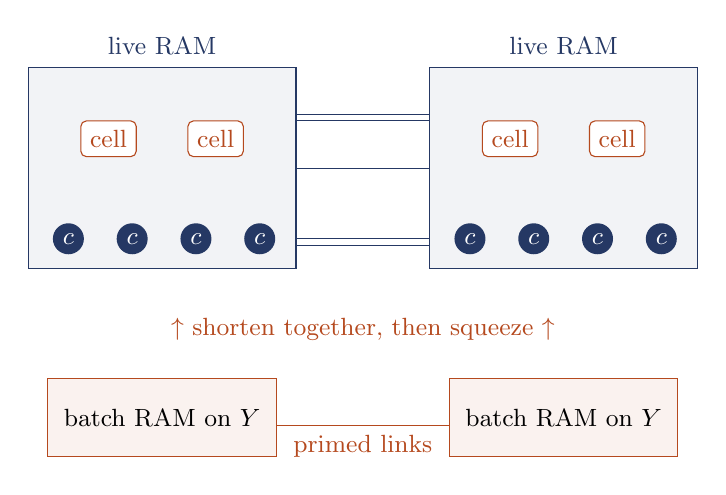
\begin{tikzpicture}[x=1cm,y=1cm,font=\small]
  \definecolor{live}{RGB}{37,56,100}
  \definecolor{primed}{RGB}{181,73,30}
  \foreach \offset in {0,5.1} {
    \begin{scope}[xshift=\offset cm]
      \draw[live,fill=live!6] (0,0) rectangle (3.4,2.55);
      \node[live,above] at (1.7,2.6) {live RAM};
      \foreach \x in {1.02,2.38}
        \node[draw=primed,text=primed,fill=white,rounded corners=2pt]
          at (\x,1.65) {cell};
      \foreach \x in {0.51,1.32,2.13,2.94}
        \node[circle,fill=live,text=white,inner sep=2pt] at (\x,.38) {$c$};
      \draw[primed,fill=primed!7] (.25,-2.38) rectangle (3.15,-1.40);
      \node at (1.7,-1.89) {batch RAM on $Y$};
    \end{scope}
  }
  \foreach \y in {.30,.38,1.275,1.88,1.96}
    \draw[live] (3.4,\y) -- (5.1,\y);
  \node[primed] at (4.25,-.77) {$\uparrow$ shorten together, then squeeze $\uparrow$};
  \draw[primed] (3.15,-1.99) -- (5.35,-1.99)
    node[midway,below] {primed links};
\end{tikzpicture}
\caption{What gets replayed (two of many teams). A batch RAM sees even the code for the live
simulation but uses it only as slot addresses, not as code. Pieces from many primed teams can end
up inside the same cell, and the cells migrate to live teams as determined by a public ledger.}
\label{fig:replay}
\end{figure}


It is important that we need to process more than the exterior links here. New RAM
transcript wires in the replay may carry width even larger than all the ports we started
with! So there will be two scheduling theorems.

\begin{enumerate}
\item We pack the primed RAM computations together by repeated geometric shortening
(\S\ref{sec:packing}). This squeezes nearly all of their new wires into little cells (very cheap to
compute \emph{privately} in the live RAM). Costs to describe a wire bundle \emph{publicly} are only
polylogarithmic; large widths amortize the overhead. The primed exterior links are
carried along unharmed; too few and dispersed for bulk shortening, their ends can
wind up anywhere.
\item We clear everything still crossing, dominated by these exterior links, by a final squeeze
(\S\ref{sec:exterior}). Total available physical capacity between teams would look about adequate but
the capacity between \emph{each pair} must suffice, plus we need breathing room. We assign
packed cells to live RAMs in a way that lets us save a constant fraction even on this
unstructured interconnection.
\end{enumerate}

\subsection{Transcript compilation}

Here is the RAM convention we use and its compiler to bit networks. The idea of sorting to
check RAM/random access is standard (see e.g. \cite{BCGTV} and references therein). Words, including
for addresses and times, have $w=O(\log(nr))$ bits with sufficiently large constant; polylog-bit
quantities can also just use several words. Our fixed programs use a constant number of
registers. A tick does elementary work on constantly many words (ordinary integer/bit
operations on bounded words, one memory probe, one binary choice, branching); the initial
state can include size/index parameters. In live programs only, allow calls to a fixed private
subroutine on $b\le n^{1/2}$ consecutive memory words read, with its own nondeterminism (can
reject); cost $b+1$ ticks (call parameters, including $b$, already determined by register state
before these ticks). It may validate declared outputs in those words; it need make no changes.
Bound its time by $n^{50}$ multitape steps. We count accepting paths.

Compile onto $t$ buckets ($t$ power of two); initial memory is the disjoint union of $O(B)$
given bits per bucket (one bit per word, other memory zero). The machine gets $tB$ ticks for
ordinary programs; halve for those with private calls, using in that case $B\gg n^{1/2}$. Time
out by rejection. Then:

\begin{itemize}
\item The contraction with these inputs gives the acceptance count, each path counted
exactly once.
\item The compiler uses $\widetilde{O}(B)$ incident internal bits per bucket, in polylog many cable
descriptions. Cables are between indices related by one-bit flip or predecessor/successor.
We assume $B\le n$, $t$ polynomial in $nr$.
\item Layout of compiler cables at any bucket is computable in polylog time. Bucket functions
are counts of local validators.
\end{itemize}

Indeed give each bucket $B$ consecutive ticks, passing register state (and halt status propagated
canonically, time used, etc.) to the successor. If a call will not fit, pass before it; wasted
ticks thus cannot defeat the halved budget. Guess previous contents at all probes (including
for the memory reads of a private call), producing records by address and time of previous
and resulting words. Include initialization records for given bits at time zero (previous word
zero) and canonical dummies, padding to a fixed common power of two $O(B)$ records per
bucket. Sort deterministically by address and time (dummies last), with Batcher bitonic
sort \cite{Batcher}. This uses $O(\log^2(tB))$ parallel layers in which partners differ in one index bit of
the entire record array; across buckets this gives one full exchange between XOR neighbors.
At the end, exchange also boundary records with successive buckets; check previous values
by immediate predecessors at same address (default zero). Thus for any accepting path all
guesses of probe values are forced. All internal shared bits have canonical values. These
operations are local checks given incident cable bits; deterministic wiring and unused bits
do not add multiplicity. We require simple indexing conventions (given sizes and bucket
ordinal) for assigning initial addresses, as used below. Validators without private calls have
ample implementations in $n^{15}$ local tape time (even scanning all local data for individual
references and using school arithmetic); those with calls fit in $n^{80}$. Here we already take $\rho$
small so polylogs used by fixed routines are, say, $O(n^{.01})$.

\subsection{Choice of scales}

Here and below there is generous polynomial slack except in the total width of exterior
links. Packing (\S\ref{sec:packing}) gives fixed constants $K_0 \ge 2$ (number of networks combined per epoch),
$C_\ast \ge 2$ (per-cell growth factor including incidence), independent of resource exponents. Use
\[
  T=\lfloor\tau\log n\rfloor,\qquad R=K_0^T,\qquad \xi=\tau/3,\qquad X_0=rn^{1-\xi}.
\]
Make $\tau >0$ so small that $R,C_\ast^T,2^T\le n^{10^{-7}}$. Then take $\rho >0$ small. Every fixed polylog
overhead used in the construction and its estimates may be absorbed in $O(n^{\xi/100})$, taking
account also of combined overheads; the fixed powers of logs in our algorithms are independent
of $\rho$. We can supply all size parameters; no real arithmetic is intended. Use floors or ceilings
as needed.

Each processor has fields of $\lfloor n^{.2}\rfloor$ literal and that many pin bits. Pin inputs fit distributed
over team one (pin length $\poly(M)\ll r$); pad all fields. For each other team use $\lfloor n^{1-\xi}/R\rfloor$
exterior links per processor, physically between equal processor numbers; their total incident
at a team is at most $X_0$. Team RAMs use the compiler with $t=r$, $B=\lfloor n^{1-\xi/2}\rfloor$, private
calls allowed, initializing these three kinds of fields as input bits, memory order by processor.
All fields and compiler cable ends together fit the $n$ ports per processor. Literal header
includes validator program, parameters and processor name. There is no need for a program
to compute its own code: these same literal bits are also inputs. Large advice, including
entry algorithms, can likewise be distributed. All validators themselves use fixed code (with
universal interpretation within the RAM program as needed, timed in ticks, e.g. to use the
entry algorithms).

\paragraph{Batch algorithm for primed teams.}
Fix all primed literal, pin and exterior bits for one
primed team. Given also a parameter exponent vector for that team (total degree $r(2n-1)$),
count its coefficient in the primed execution of the team. There is a $\widetilde{O}(rn)$ ordinary RAM
for this. Guess all interior links, use the resulting processor inputs $x$ (padded as in defining
$F$) to specify the $r$ requested slots of the degree-$n$ output, and guess one ordered parse per
slot. Validate that leaves match the specified $Z$-monomial, and aggregate parameter uses,
checking the given histogram. Indeed palettes and parameter names have size polynomial
in $M$ (number of possible names), and we can aggregate by random access to counters;
initialization and final histogram check outside the parse loop are cheap. One parse costs
$\widetilde{O}(n)$, using regularly numbered gates and parameters, stack traversal and bit array checks.
Also the per-processor layout of live interior links can be interpreted within this time, using
the regular compiler layouts (even the $R$ exterior fields have simple address arithmetic).
Therefore the full primed contraction with fixed pin has its coefficients given by contracting
such batch networks along the primed exterior links and adding exponents across teams.

Compile this RAM with $B=\lfloor n^{.2}\rfloor$ and $t=\widetilde{O}(rn^{.8})$, same at all teams
and with sufficient
ticks. Group initial-memory inputs in lists: exterior list for each other team, ordered
by processor number then bit number (shared at both teams), literal and pin fields, and
exponent inputs. Chunk each list separately into blocks of at most $B$ bits so exterior-list
cables are attached between corresponding initialization chunks (one bucket per chunk on
each side). Addressing is regular and all descriptors per bucket including compiler incidence
fit polylog words. Only compiler cables, \emph{not} exterior lists, are charged during bulk shortening.
Primed validators are used as little boxes: no need to reveal their local probes or choices in
a public description. They don't run the live validators; this keeps their private cost very
small. All these networks are placed next.

\section{A geometry for iterating the saving}\label{sec:packing}

The following lemma implements bulk shortening. It does not depend on the functions in
the boxes. We detail algorithmic bounds because our diagonal program must itself recreate
the schedules, inside its tick budget.

\begin{figure}[htbp]
\centering
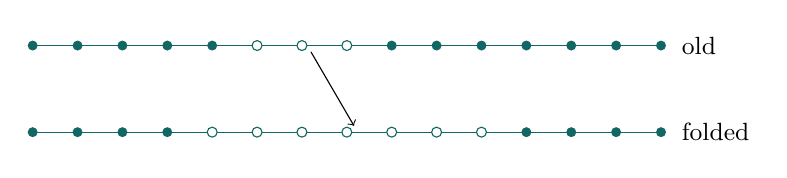
\begin{tikzpicture}[x=.57cm,y=1cm,font=\small]
  \definecolor{lamp}{RGB}{18,102,99}
  \foreach \y/\first/\last/\name in {1.1/5/7/old,0/4/10/folded} {
    \draw[lamp] (0,\y) -- (14,\y) node[right=4pt,text=black] {\name};
    \foreach \x in {0,...,14} {
      \ifnum\x<\first \fill[lamp] (\x,\y) circle (1.8pt);
      \else\ifnum\x>\last \fill[lamp] (\x,\y) circle (1.8pt);
      \else \draw[lamp,fill=white] (\x,\y) circle (1.8pt);
      \fi\fi
    }
  }
  \draw[->] (6.2,1.02) -- (7.16,.08);
\end{tikzpicture}
\caption{One cycle, cut open. White lamps are forgotten. When making a new site at a nearby
height we can inherit all specified lamps by increasing the radius by a constant. Only boundedly
many old site labels per height can compete to feed one such label.}
\label{fig:window}
\end{figure}


\paragraph{Windowed host.}
Fix shortening of fraction $\nu >0$ in dimension $D$ as above, exact with
integer selector budget. Put $q=2^D$. Take $q$ cycles of length $\ell$ and sites with height in
$(\mathbb{Z}/\ell)^q$. Additionally each site has $q$ partial binary lamp strings, one on each cycle: all lamps
specified except those in a window of radius $a$ at its current height in that cycle. Thus the
number of sites at radius $a$ is
\[
  V_a= \ell^q2^{q(\ell-1-2a)}.
\]
All radii used will be $O(\log n)$, with $\ell$ of order $\log r$, much larger. Neighbor steps change
height by one on one axis and agree on overlapping known lamp bits. Radius zero looks like
a cyclic butterfly: passing a lamp frees one to switch the bit there (compare cube-connected
cycles \cite{PVCC}). Increasing radius lets us perform local Euclidean geometry on heights and pay
for it by a little folding in lamp space.

During an epoch allow rational heights (bounded denominators), windows centered at
floors; cables of height displacement norm at most one, with labels agreeing on joint domain.
Cost for a charged bit is the Euclidean displacement norm using short cyclic lifts. Bits
local at a site are free and remain local. Uncharged cables take no part; one can work with
external terminals attached.

For a placed network at radius $a$, let $W$ be total charged length, and
\[
  Z=\sqrt{V_a}\left(\sum_x z_x^2\right)^{1/2}
\]
where $z_x$ counts incidences at actual site $x$ of charged bits of positive length. A public record
(descriptor) can name a box, a port interval, a cable end, etc., with constantly many indices.
Also track expanded load at each site: public records with, in addition, incident widths
(even uncharged), local slot bits and data, and multiplicities of local block factors implicit in
bundled descriptions (including identity/reblocking operations, but fixed tables or validators
treated as boxes, counting input widths not private evaluation time).

\begin{lemma}[epoch]\label{thm:epoch}
There are constants $K_0 \ge 2,\lambda >0,C_\ast \ge 2$ and a constant radius
increment with the following property. Combine $K_0$ networks at the same radius with integral
heights and only neighbor steps charged. They can be replaced by a sum at the increased
radius (allowing this much window room), again integral with neighbor steps. In every
summand,
\[
  W_{\mathrm{out}}+\lambda Z_{\mathrm{out}} \le K_0\left(\tfrac12\max_i(W_i+\lambda Z_i)+O(V_a)\right).
\]
Largest per-site public record count (including old boxes and new) and similarly expanded
load, measured with one added, grow by factors at most $C_\ast$. The summands are indexed by
successive profiles; given these as reached, public work per summand is near-linear in public
record count plus $V_a$ (allow fixed polylogs of total sizes, including $V_a$, expanded loads and
names in use), not linear in expanded widths.
\end{lemma}

\begin{proof}
Assume throughout $a\le \ell/4$ with room, as in use. We give a step that combines $K$
networks, and repeat for a fixed $b$ steps on a $K$-ary tree, $K_0=K^b$. Here $b$ is chosen first;
in particular all bounded geometric types and grids in the steps can be fixed before $K$ is
chosen.

\paragraph{Motion.}
Apply independently to each incoming network a signed permutation of axes and
uniform shifts of the heights on a fixed rational grid, transporting lamps using the same
reindexing and reflection and the integer parts of shifts. XOR the lamps by uniform strings
(one whole pattern per motion). Take permutations also uniform with all signs; this is
initially a randomized description, to be fixed deterministically. Increase the window radius
by two so new known lamps indeed come from old ones. A cable retains displacement up
to signed permutation, and agreement on lamps. Any fixed such motion is bounded-to-one
since only boundedly many known bits can be lost and heights are carried isometrically.

Bin all charged positive-length segments, oriented in advance, by exact midpoint height,
lamp label for that midpoint at radius another two larger, and exact displacement vector.
Either endpoint provides this label, since all requested lamps are known to both. There are
$O(V_a)$ bins (include all signed variants), since we have only constantly many such rational
displacement vectors and fixed grids. Indeed start with integral heights, take the shift
grids containing all previous heights and possible midpoints, and all geometric replacements
below also use only rational combinations, with denominator bounds fixed at each step. In
expectation, bin counts (counting width bits) are invariant under signed permutations on
the vector part \emph{alone}: conditional on displacement, midpoint is uniform on its grid and
lamps are independently uniform.

\paragraph{Pairing in orthogonal tuples.}
Index axes by binary strings of length $D$. The $D$ signed
permutations
\[
  A_j e_x= (-1)^{x_1+\cdots+x_{j-1}} e_{x^{(j)}}
\]
(where the superscript flips bit $j$) are symmetric involutions anticommuting pairwise. Thus
$A_j v$ are pairwise orthogonal for each $v$. In each bin, divide width into $D$ equal integer
pools (leaving remainder alone). For each seed bin $s$, use pool $j$ of bin $A_j s$ (acting just
on displacement); these requests are disjoint. Take the minimum available width, rounded
down to a multiple of shortening width $m$, in all these directions. We have crossings: use the
grouped identity with profiles there, at midpoint, taking as frame the vectors $A_j v/2$ (seed
displacement $v$), hence scaling by $\| v\| /2$. This saves fraction $\nu$ of length served (decrease
the fraction if needed). Increase all radii to midpoint label radius plus two, so all new
sites get labels from the midpoint, matching moved endpoints, and all segments again have
the required form. Unserved bits stay. As throughout, different objects at the same site
can retain their own boxes, using free local wires. Profile sums here are exact expansions
with any other slots left open, so after profiles are specified we may expand anew in ways
depending on the result.

The per-site growth at each step is bounded (allow factors depending on $K$ here). A
bin involves only boundedly many nearby possible sites: heights within bounded distance
on fixed grids, and labels constrained except for boundedly many bits. Conversely only
boundedly many bins affect a site, for the same reasons. We used also bounded fibers of
a motion. Pool intervals meet cable descriptions in only linear complexity (order cables
deterministically); at crossing terminals concatenate all relevant widths before applying the
grouped gadget. Thus new descriptors are locally linear in input descriptor counts plus
constant, with profile integers themselves just counts. Expanded load grows likewise relative
to expanded load (gadget size and work counted here linear as positions, not necessarily as
tape time).

\paragraph{Cost and concentration.}
For a step let $y$ be the sum of bin count vectors over incoming
packs (networks), and $\bar y$ its expectation. With bin invariance, ideal counts would achieve
full service apart from rounding. Thus unserved length is bounded by
\[
  C\left(V_a+\sqrt{V_a}\,\lVert y-\bar y\rVert_2\right),
\]
as loss at one seed is bounded by constant plus a constant times the sum of absolute
deviations at its requested bins; use Cauchy--Schwarz. Here and below $C$ can depend on $b$
and the fixed geometric construction but not $K$. For one pack, any motion gives bin-vector
norm $\le CZ_i/\sqrt{V_a}$ (bounded fibers and nearby sites as above). Therefore deterministically
we can obtain
\[
  \sqrt{V_a}\,\lVert y-\bar y\rVert_2 \le C\sqrt{K}\max_i Z_i
\]
by not exceeding the expected squared norm of the deviation (independence). Furthermore,
$\sqrt{V_a}\,\lVert\bar y\rVert_2\le C\sum_i W_i$ by uniformity over positions with lamps and a
positive minimum length.
New incidence norm $Z'$ is at most $C\sqrt{V_a}\lVert y\rVert_2$ by bounded geometry again (counting new
charged bits, even control, per served width). Consequently
\[
  \begin{aligned}
    W'/K &\le(1-\nu)\max_i W_i+ C(K^{-1/2}\max_i Z_i+V_a), \\
    Z'/K &\le C(\max_i W_i+K^{-1/2}\max_i Z_i).
  \end{aligned}
\]
\paragraph{Fixing motions efficiently.}
Use conditional expectations, as standard (cf. \cite{Raghavan}). Fix
one motion at a time, enumerating the permutation, signs and heights (poly in $\ell$); then
determine its XOR pattern bit by bit. All comparisons of conditional objectives are rational
with polylog bit size: common denominators can use the numbers of completions/products
of choices. Here are details to see near-linear work. For given permutation/signs and shifts,
form the moved count vector with XOR bits yet unfixed taken zero. Its squared norm is
independent of the remaining XOR pattern (permutation of bins). To form the conditional
mean vector, average each bin class with displacement, center and all bits unaffected by
remaining XOR choices fixed; this distributes its sum uniformly in that class. These are
list operations using sorting/prefix sums over all possible bins and cable descriptors. They
therefore give the needed means and second moments (square-norm expectations), even
averaging over permutations and shifts when those are not specified. For different packs use
independence for inner products. This implements the choices in the bound, with no need
for any individual bit of a payload cable.

\paragraph{Rounding.}
After $b$ steps round heights to integers with common offset then floor, routing
a segment by successive coordinate steps. As before increase window radius by a constant
(say six); along the short route all specified lamps can be inherited from common knowledge
of both endpoints. Mean length with uniform offset in the unit cube is now bounded by $\sqrt{q}$
times previous length, by comparison with $\ell_1$. Fix minimizing offsets (enumerate fixed grids),
with this bound. Incidence norm and site loads incur at most constant factors by bounded
geometry. Choose $b$ so $\sqrt{q}(1-\nu)^b<1/8$. Iterate the two inequalities above (equivalently
normalize by number of starting packs under each subtree). After rounding and dividing by
$K^b$, length is bounded by
\[
  \tfrac18\max_i W_i+ O(K^{-1/2})(\max_i W_i+\max_i Z_i) + O(V_a);
\]
incidence norm similarly but with $O(1)$ instead of $1/8$. Thus choosing $\lambda$ small, then $K$ large,
proves the lemma; public work and descriptors have the claimed bounds by the lists and
bounded local operations.
\end{proof}

\paragraph{Application to batch networks.}
Take minimal $\ell$ with $2^{q(\ell-1)}\ge t$ for the primed batch
RAMs. At radius zero place buckets by Gray coding their binary numbers (binary-reflected:
XOR number with its right shift), padding into the lamps at height vector zero. Thus
successors differ in one bit, XOR neighbors in at most two. Route all charged cables by
paths changing single bits: take the height on the appropriate cycle around to the lamp
position, then back with that bit changed (treat other passing bits as unchanged, specifying
the originally omitted height-zero bits by zero as needed). Insert identity operations. This
costs polylog factors and causes at most polylog local growth within one team. Indeed at
any intermediate site only polylog original buckets are possible (only constantly many bits
changed or unspecified), routes have polylog length and each bucket polylog descriptors.

Thus for one input pack, descriptors per site number $\widetilde{O}(1)$ and expanded load is
$\widetilde{O}(n^{.2})$.
Also
\[
  V_0=\widetilde{O}(rn^{.8}),\qquad W+\lambda Z=\widetilde{O}(rn).
\]
Iterate Lemma~\ref{thm:epoch} through $T$ epochs combining all $R$ packs, tracking profiles. This requires
radius $O(T)\ll \ell$. After normalizing output per original team we have on every summand
\[
  O(2^{-T})\,\widetilde{O}(rn)+O(V_0)=o(X_0)
\]
as a bound on charged length. At this point call the sites cells. Between cells, total width of
shared bits, including primed exterior, is at most
\begin{equation}\label{eq:intercell}
  RX_0/2+o(RX_0).
\end{equation}
The small literal and pin fields (and exponent lists) attach separately as fixed inputs once
supplied by a ledger.

Each cell has $O(n^{.001})$ descriptors and $O(n^{.25})$ expanded load. All public reconstruction,
starting from team descriptions, and given successive profiles, costs $O(rn^{.82})$ ticks even for a
single live RAM reproducing everything. Indeed there are at most $O(RT)$ epoch applications
and the per-site descriptor bound holds throughout; public algorithms use polylog overheads,
with initial record lists and routes generated by regular indices and colors, lamps and counts
fitting polylog bits (by colors here we mean indices of fixed shortening entries, \emph{not} their
field values). Profile sequences fit the same bound in bits; e.g. allocate profile counters in
deterministic order as the public replacements are made, reading from a tape, rejecting
malformed or out-of-range profiles and requiring zero padding.

\section{Clearing exterior links}\label{sec:exterior}

Here we adapt the striking square scheme of \cite[\S2]{Anthropic3SAT}---including its two-layout crossing
step, the $11/12$ saving and grid and balancing ideas---to transcript replay. We need the
integral form across characteristics (cf. Clifford and sums-of-squares literature \cite{HWY,Hrubes}, and
the powerful integral construction \cite{Khoruzhii}), tight \emph{pairwise} capacities, uniquely checkable choices,
and near-linear public reconstruction (cf. also the balancing in \cite{ETHfalse}).

Let $d=R^{16}$ (new notation in this section), $Z_0=d^2$. Give each cell a label in $[d]^2$.
Do this so that orienting intercell cables by a fixed rule first, each ordered pair of labels
(including equal) gets width at most
\[
  RX_0/(2Z_0^2) + o(RX_0/Z_0^2).
\]
Indeed under independent uniform labels this holds in expectation by \eqref{eq:intercell}. Variance for
any pair of labels is at most $O(RX_0 \cdot n^{.25})$, since only cables meeting a common cell need be
counted for deviations, and cell loads are bounded. Thus deterministically not exceeding
expectation of sum of squares of deviations suffices ($r$ dwarfs any polynomial in $n$).

Again choose by conditional expectations. To give explicit public cost bounds: maintain
the means and variances for pair totals separately, trying each label for the next cell. Mean
updates use incident cable records; variance is a sum of covariances over meeting pairs of
cables including self-pairs, so update at pairs including an incident cable and use probabilities
given by equality and uniform probabilities at at most three vertices. Thus with $O(n^{.001})$
incident records per cell even $O(Z_0^4 n^{.003})$ such polylog-arithmetic work per cell suffices.
Parallel cables need not be expanded.

Pad to equal multiple-of-three width on every ordered pair, pinning dummies (if there
are no wires, allow width zero). Total padded width $P\le RX_0/2+o(RX_0)$. All but $O(P/d)$
bits run between corners differing in both coordinates. Make packets in each rectangle
joining its two diagonals (opposite label pairs), taking three consecutive bits on each. Do
this separately for lexicographically forward and backward wires.

A packet tensor on the four corners has the identity
\[
  \mathbf{1}_{x=y}\mathbf{1}_{i=j} = \sum_{z=1}^8 A(x,i,z)B(y,j,z) + \sum_{z=1}^8 C(y,i,z)D'(x,j,z)
\]
with integral fixed arrays, where $x,y$ are indices of size eight at one pair of opposite corners
and $i,j$ at the other pair. Indeed on exterior algebra of four generators take $P_x$ to be the
eight wedge and contraction operators, $Q_y$ the same with wedge and contraction exchanged.
Use even-to-even entries $(j,i)$ of $Q_y P_x+P_x Q_y=\delta_{xy}I$, factoring through odd states.

Group labels by one coordinate into $d$ symbols. For each packet there are two symbols
involved. Between them use one shared selector bit choosing the term. For the term factored
along this split send three rank bits. For the other term use six (trivial rank bound; one side
gives both indices to the other). Add the two possibilities for coordinate choice: given term,
cost with selection is four for one grouping and seven for the other. This is a real saving
since packing two unaltered diagonals would cost six either way.

Specifically add to a common ledger the histogram of selectors within each rectangle and
orientation. Use consistent indexing of corners throughout such a class. Choose grouping
minimizing total cost given histograms (canonical ties; direct wires between symbols for
nonpacket bits), so total between-symbol widths are at most
\[
  (11/12)P+O(P/d).
\]
\begin{figure}[htbp]
\centering
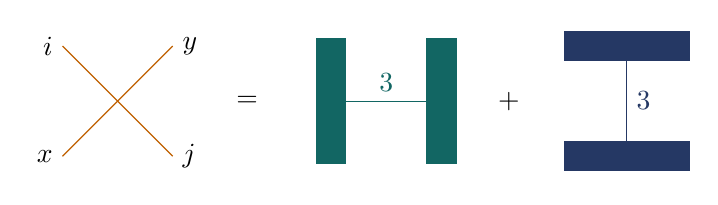
\begin{tikzpicture}[x=.7cm,y=.7cm]
  \definecolor{vertical}{RGB}{18,102,99}
  \definecolor{horizontal}{RGB}{37,56,100}
  \draw[orange!75!black] (0,0) node[left,text=black] {$x$} --
    (2,2) node[right,text=black] {$y$};
  \draw[orange!75!black] (0,2) node[left,text=black] {$i$} --
    (2,0) node[right,text=black] {$j$};
  \node at (3.35,1) {$=$};
  \foreach \x in {4.6,6.6}
    \fill[vertical] (\x,-.14) rectangle ++(.55,2.28);
  \draw[vertical] (5.15,1) -- (6.6,1) node[midway,above] {$3$};
  \node at (8.1,1) {$+$};
  \foreach \y in {-.27,1.73}
    \fill[horizontal] (9.1,\y) rectangle ++(2.28,.55);
  \draw[horizontal] (10.24,.28) -- (10.24,1.73) node[midway,right] {$3$};
\end{tikzpicture}
\caption{Two terms for a packet (numbers in bits). For either term one of the two ways of grouping
costs three, the other at most six, before adding selectors. One grouping will be chosen globally
using selector histograms.}
\label{fig:packet}
\end{figure}


For a histogram, costs by symbol pair are public; actual selector bits need be available only
to the two symbols handling the rectangle. On shared strings use selector bits first and
check histograms to know the rest of the layout, enforcing equality bits and applying factor
tables within symbols. Even though the grouping can change with histograms, summing
gives exactly the desired packet contraction: for each choice of all selectors the same term
tensors are used (rank-cable contraction gives exactly the term for either grouping). Also
the raw load per symbol in padded wires and incident packet positions is $O(P/d)$ by equal
padding.

Assign symbols to live teams, again by conditional expectations. For each unordered
pair of distinct teams the load under independent assignment has expectation at most
$2((11/12)P+O(P/d))/R^2$ and variance $O(P^2/d)$ (meeting pairs). Also the number of
symbols assigned to a team has mean $d/R$, variance at most $d$. Control sum of squares of
deviations for both by normalizing separately by $(P/R^2)^2$ (omit if $P=0$), $(d/R)^2$; resulting
expectation summed is $o(1)$. Thus simultaneously:

\begin{itemize}
\item each distinct team pair gets at most $(11/12+o(1))X_0/R$ bits;
\item each team's padded load to process, including symbols assigned to the same team
communicating locally, is $O(X_0)$.
\end{itemize}

All operations on histograms and totals for ordered pairs, rectangles, symbols or team pairs
can certainly be done in $O(d^{20})$ work times polylogs, besides manipulating lists of all the
cable descriptions (form intervals by sorting and prefix sums, keeping track of cell endpoints).
For assignment of symbols only the graph on $d$ symbols with weights by pair is needed, so
naive conditional computations (covariances and means as before) more than fit.

\section{Assembling the programs}\label{sec:assembly}

Here we finish Lemma~\ref{thm:replay}. We include details since one needs both resource bounds and
exact counts (in particular no multiplicity for \emph{proofs} that a layout is legal). All scheduling
routines use fixed formats and deterministic tie breaking.

\paragraph{Common ledger.}
Given the lemma data, use live processors, literals (including advice)
and layouts as in \S\ref{sec:replay}. Reserve prefixes on physical exterior bundles between every pair of
teams, so that live team RAMs have initial copies of the same guessed ledger: check equality
at each team, giving equality throughout. The ledger includes a branch bit; in the unit
branch require all other exterior-link bits zero (including unused ledger), and team one tests
the live pin for equality to $\ast$ (decode $\ast$ from advice there). No private guessing in team
RAMs for that branch, hence contribution $e_\ast$ exactly.

In replay branch include:

\begin{itemize}
\item copies of \emph{all} literal fields checked by their owners, primed pin index $I$ (to initialize
primed pin fields), and proposed exponent vectors at every primed team;
\item epoch profiles and squeeze histograms in reconstruction order;
\item later-used color subtotals at each live team: total uses of each fixed table value in its
own part of the contraction as expanded. These colors are drawn from a fixed finite
list of table entries of shortening and packet gadgets, tracked by their names. Other
operations just count (e.g. enforce selectors and routing, or contribute one per local
accepting path).
\end{itemize}

Weights, programs for computing matrix entries, and fields and specialization data need
not be small in $n$; they need only have $\poly(M)$ bits, and are easily carried in literals and
accessible in reconstructed arrays (in particular give team one all data needed for final scalar
operations). Live processors hold only their own shares of large literal data.

Use fixed padded ledger room, say $\lceil rn^{.90}\rceil$ bits per physical team pair. This easily
suffices by the reconstruction bounds and $Rrn^{.2}$ literal volume. All counters of layout sizes,
table uses, etc., need only polylog bits as all expanded sizes are polynomial in $rn$. Check
all formats, ranges, sizes and padding, to enforce canonical descriptions. All sizes used
as capacities and public padding dimensions can themselves be supplied unsurprisingly in
advice, which is fixed in defining $F$. In particular program headers give compiler parameters,
clocks and field lengths. Corrupt ledger or nonconforming computation can always just
reject.

Each team RAM reconstructs public schedules, and checks and accesses ledger data as
needed, in $O(rn^{.95})$ ticks by the bounds. It learns the symbol grouping, assignment, and
shared string lengths for squeeze. Pack these shared strings canonically between distinct
team pairs, using physical link bundles ($r\lfloor n^{1-\xi}/R\rfloor$ bits available per pair before ledger).
They fit, by the $11/12$ bound. All unused bits are enforced zero.

\paragraph{Inside a team.}
The team's job in contraction is exactly its assigned symbols, including all
cells therein. For squeeze it handles only its incident shared strings (guessing each same-team
shared string once), computing also unshared packet and padded data (dummy pins use zero).
This is straightforward bit-level contraction: guess local indices once, check all selectors and
histograms for the involved rectangles, equality/delivery to cell slot arguments, and attach
the designated packet table entries to the path. Work including grouping individual wire
bits for cell calls costs $\widetilde{O}(X_0)$ plus public reconstruction: the raw expanded squeeze cost
per team is $O(X_0)$, we can translate positions through padded intervals by binary search in
public cable arrays, and use ordinary addressed memory, or sorting, for reordering.

Call the private subroutine on every assigned cell, supplying its public descriptors,
intercell slot bits, and data fields for its input positions (batch literal, pin and histogram
inputs for primed RAMs), plus declared cell totals of colors (which it checks). Total of such
primed RAM initial data fields, not counting primed exterior, over the entire construction is
$O(Rrn^{.2}+R\poly(M))$, since folding and placing do not duplicate any initial box. Thus call
overhead and outer RAM work of preparing arguments fits the bounds (assemble by records
by cell name). Each call fits in $n^{1/2}$ words by per-site estimates; we do not pass the bits
on cables \emph{inside} a cell. Privately expand and process the local contraction, guessing those
internal bits, testing local constraints and reblocking and executing local batch-compiler
bucket validators (one per hosted bucket), so multiplicities are the path counts. This fits
the private time cap per call: with $O(n^{.25})$ expanded load, even generating explicit arrays of
local slots and uses with polylog addressing overhead, using repeated scans for lookups and
selector subsequence indices and school arithmetic for bounded integers, takes, say, $O(n^{10})$,
besides validator work ($O(n^{15})$ per bucket). There is no arithmetic in a huge finite field here:
only tally color names. Team RAMs total these counts (also their squeeze packet colors)
and check their ledger subtotals.

Finally, let $\lambda$ denote the product of all recorded color values. Team one computes
this weight by powering from subtotals. Fix a prime-field linear projection $\pi$ from the
specialization field to the prime field with $\pi(1)=1$, part of advice. With $\mu$ the sum of
proposed team exponents and $H$ the live pin, team one inserts
\[
  \pi(\lambda)\,(W_\mu)_{I,H}
\]
as path multiplicity modulo $p$. Implement as ordinary nondeterminism by allowing as many
choices as the representative of $\pi(\lambda)$ (guess a smaller nonnegative integer canonically) and
running the matrix entry path procedure. All operations on the aggregated values are of
cost $\poly(M)$, or that times $R$; standard polynomial overhead simulation suffices.

Thus a live team fits in $O(rn^{.95})+\widetilde{O}(X_0)$ ticks (increasing the first exponent a little, say
to $.96$, if needed), inside its compiler limit. Private, tick and validator limits may always
be enforced, with rejection on malformed data. They do not exclude any contributing
computation.

\paragraph{Accounting identity.}
Hold fixed $I$ and the team exponent proposals. By contraction,
summing fully expanded terms with color weights gives exactly the corresponding batch
count: squeeze, then each shortening, can be summed out in reverse order, with all these
inputs fixed. In this expanded sum a term specifies profiles and histogram choices, internal
indices, and paths where boxes count. Live counting realizes precisely this enumeration (up to
the final weight multiplication just described). Indeed any such term meeting the contraction
checks gives unique additional ledger data such as color subtotals, unique additional physical
assignments and transcripts by their checks and deterministic layouts; conversely accepting
paths must correspond (including the private local path choices). Projection $\pi$ commutes
with summing these weighted terms, and batch counts were prime-field to begin with.

Summing also over the proposals giving total $\mu$, one therefore gets
\[
  ([X^\mu]F_I(Y(X)))\,(W_\mu)_{I,H}.
\]
The symbolic row has degree $Rr\le L/(2n)$, so all exponents used are in range. Adding over
$I,\mu$ and including the unit branch proves precisely Lemma~\ref{thm:replay}. This finishes the proof of
separation.

\paragraph{Low degree application.}
To indicate the flexibility of the witness, even clique polynomials
can show such bounds with only polylogarithmic degree. In each fixed characteristic take
ordinary clique (monomial is product of edge variables) on $N$ vertices, clique size $\lceil \log^A N\rceil$ for
a sufficiently large constant $A$. This is in $\mathrm{VNP}$, and has border complexity
$\exp(\Omega((\log N)^{5/4}))$.
To see this, recall the elementary projection: encode a sum over compatible choices at $k$
sites (pairwise constraints, unary weights) by one part of vertices per site plus a singleton
for attaching all unary weights by edges. Force selection of one per part by zero within
parts; extra singleton parts pad the clique size. Use constants for compatibility. In the
no-shortening proof apply this directly to the partition polynomial $g$ with $n$ taken a small
fixed power of $N$ (the same balanced-cut proof bounds $g$ itself). With shortening, take $n$ a
power of $\log N$ large enough for the stretch theorem to suffice; encode the tableau sum for
$f_n$. For example, sites represent Boolean values and also satisfying tuples for individual local
constraints, edges matching constraint arguments to their values; attach variable weights
at the $x$ sites. This uses only polynomially many sites and vertices in $n$, so fits with $A$
large. As before projection after homogenization suffices even for degree-component border
lower bounds. This growing-parameter conclusion is to be distinguished from hardness in
parameterized models (cf. \cite{be}).

\begin{thebibliography}{99}
\small\raggedright
\bibitem{AgrawalVinay}
Manindra Agrawal and V. Vinay. Arithmetic circuits: A chasm at depth four. In \emph{49th Annual
IEEE Symposium on Foundations of Computer Science}, pages 67--75, 2008.

\bibitem{AKV20}
Noga Alon, Mrinal Kumar, and Ben Lee Volk. Unbalancing sets and an almost quadratic lower
bound for syntactically multilinear arithmetic circuits. \emph{Combinatorica}, 40(2):149--178, 2020.

\bibitem{Batcher}
K. E. Batcher. Sorting networks and their applications. In \emph{Proceedings of the Spring Joint
Computer Conference}, volume 32 of \emph{AFIPS Conference Proceedings}, pages 307--314, 1968.

\bibitem{BaurStrassen}
Walter Baur and Volker Strassen. The complexity of partial derivatives. \emph{Theoretical Computer
Science}, 22(3):317--330, 1983.

\bibitem{BCGTV}
Eli Ben-Sasson, Alessandro Chiesa, Daniel Genkin, Eran Tromer, and Madars Virza. SNARKs
for C: Verifying program executions succinctly and in zero knowledge. In \emph{CRYPTO}, pages
90--108, 2013.

\bibitem{BDS24}
C. S. Bhargav, Sagnik Dutta, and Nitin Saxena. Improved lower bound, and proof barrier, for
constant depth algebraic circuits. \emph{ACM Transactions on Computation Theory}, 16(4):23:1--23:22,
2024.

\bibitem{be}
Markus Bläser and Christian Engels. Parameterized Valiant's classes. In \emph{14th International
Symposium on Parameterized and Exact Computation}, volume 148 of \emph{Leibniz International
Proceedings in Informatics}, pages 3:1--3:14. Schloss Dagstuhl--Leibniz-Zentrum für Informatik,
2019.

\bibitem{BGS}
Mark Braverman, Sumegha Garg, and Ariel Schvartzman. Coding in undirected graphs is either
very helpful or not helpful at all. In \emph{8th Innovations in Theoretical Computer Science Conference
(ITCS 2017)}, volume 67 of \emph{Leibniz International Proceedings in Informatics}, pages 18:1--18:18,
2017.

\bibitem{Bridy}
Andrew Bridy. Automatic sequences and curves over finite fields. \emph{Algebra \& Number Theory},
11(3):685--712, 2017.

\bibitem{Burgisser}
Peter Bürgisser. \emph{Completeness and Reduction in Algebraic Complexity Theory}, volume 7 of
\emph{Algorithms and Computation in Mathematics}. Springer, 2000.

\bibitem{ApproxFactors}
Peter Bürgisser. The complexity of factors of multivariate polynomials. \emph{Foundations of
Computational Mathematics}, 4(4):369--396, 2004. Corrected version: arXiv:1812.06828v1.

\bibitem{BC2024}
Peter Bürgisser. Completeness classes in algebraic complexity theory, 2024. arXiv:2406.06217v1.

\bibitem{BCS}
Peter Bürgisser, Michael Clausen, and Mohammad Amin Shokrollahi. \emph{Algebraic Complexity
Theory}, volume 315 of \emph{Grundlehren der mathematischen Wissenschaften}. Springer, 1997.

\bibitem{BIPnooccurrence}
Peter Bürgisser, Christian Ikenmeyer, and Greta Panova. No occurrence obstructions in geometric
complexity theory. \emph{Journal of the American Mathematical Society}, 32(1):163--193, 2019.

\bibitem{BLMW}
Peter Bürgisser, J. M. Landsberg, Laurent Manivel, and Jerzy Weyman. An overview of
mathematical issues arising in the geometric complexity theory approach to
$\mathrm{VP}\ne \mathrm{VNP}$. \emph{SIAM
Journal on Computing}, 40:1179--1209, 2011.

\bibitem{CaiChenLi}
Jin-Yi Cai, Xi Chen, and Dong Li. Quadratic lower bound for permanent vs. determinant in
any characteristic. \emph{Computational Complexity}, 19:37--56, 2010.

\bibitem{Cartier}
Pierre Cartier. Une nouvelle opération sur les formes différentielles. \emph{Comptes rendus de
l'Académie des sciences de Paris}, 244:426--428, 1957.

\bibitem{CKSS24}
Prerona Chatterjee, Deepanshu Kush, Shubhangi Saraf, and Amir Shpilka. Lower bounds for
set-multilinear branching programs. In \emph{39th Computational Complexity Conference}, volume 300
of \emph{LIPIcs}, pages 20:1--20:20, 2024.

\bibitem{CKW}
Xi Chen, Neeraj Kayal, and Avi Wigderson. Partial derivatives in arithmetic complexity and
beyond. \emph{Foundations and Trends in Theoretical Computer Science}, 6(1--2):1--138, 2011.

\bibitem{Anthropic3SAT}
Claude (Anthropic). A $2^{o(n)}$ Time Algorithm for 3-SAT. Hexagon:2610.00577v1, 2026.

\bibitem{Cook71}
Stephen A. Cook. The complexity of theorem-proving procedures. In \emph{Proceedings of the Third
Annual ACM Symposium on Theory of Computing}, pages 151--158. Association for Computing
Machinery, 1971.

\bibitem{DawarWilsenach}
Anuj Dawar and Gregory Wilsenach. Symmetric arithmetic circuits. \emph{Theory of Computing},
21(14):1--32, 2025.

\bibitem{BFLY26}
Théo Borém Fabris, Nutan Limaye, Srikanth Srinivasan, and Amir Yehudayoff. Multilinear
algebraic branching programs and the min-partition rank method. In \emph{41st Computational
Complexity Conference}, volume 383 of \emph{LIPIcs}, pages 22:1--22:20, 2026.

\bibitem{Forbes2024}
Michael A. Forbes. Low-depth algebraic circuit lower bounds over any field. In \emph{39th
Computational Complexity Conference (CCC 2024)}, volume 300 of \emph{Leibniz International
Proceedings in
Informatics}, pages 31:1--31:16. Schloss Dagstuhl -- Leibniz-Zentrum für Informatik, 2024.

\bibitem{FSV18}
Michael A. Forbes, Amir Shpilka, and Ben Lee Volk. Succinct hitting sets and barriers to
proving lower bounds for algebraic circuits. \emph{Theory of Computing}, 14(18):1--45, 2018.

\bibitem{Gro15}
Joshua A. Grochow. Unifying known lower bounds via geometric complexity theory. \emph{Computational
Complexity}, 24:393--475, 2015.

\bibitem{GKSS17}
Joshua A. Grochow, Mrinal Kumar, Michael Saks, and Shubhangi Saraf. Towards an algebraic
natural proofs barrier via polynomial identity testing. Technical Report TR17-009, Electronic
Colloquium on Computational Complexity, 2017.

\bibitem{GSS}
Zeyu Guo, Nitin Saxena, and Amit Sinhababu. Algebraic dependencies and PSPACE algorithms
in approximative complexity over any field. \emph{Theory of Computing}, 15(16):1--30, 2019.

\bibitem{GKKS14}
Ankit Gupta, Pritish Kamath, Neeraj Kayal, and Ramprasad Saptharishi. Approaching the
chasm at depth four. \emph{Journal of the ACM}, 61(6):33:1--33:16, 2014.

\bibitem{Hartshorne}
Robin Hartshorne. \emph{Algebraic Geometry}, volume 52 of \emph{Graduate Texts in Mathematics}. Springer,
1977.

\bibitem{Heintz}
Joos Heintz. Definability and fast quantifier elimination in algebraically closed fields. \emph{Theoretical
Computer Science}, 24:239--277, 1983.

\bibitem{HLW}
Shlomo Hoory, Nathan Linial, and Avi Wigderson. Expander graphs and their applications.
\emph{Bull. Amer. Math. Soc.}, 43:439--561, 2006.

\bibitem{Hrubes}
Pavel Hrube\v{s}. A subquadratic upper bound on Hurwitz's problem and related noncommutative
polynomials. \emph{SIAM Journal on Computing}, 55(2):451--467, 2026.

\bibitem{HWY}
Pavel Hrube\v{s}, Avi Wigderson, and Amir Yehudayoff. Non-commutative circuits and the
sum-of-squares problem. \emph{Journal of the American Mathematical Society}, 24:871--898, 2011.

\bibitem{Hyafil}
Laurent Hyafil. On the parallel evaluation of multivariate polynomials. \emph{SIAM Journal on
Computing}, 8(2):120--123, 1979.

\bibitem{JerrumSnir}
Mark Jerrum and Marc Snir. Some exact complexity results for straight-line computations over
semirings. \emph{Journal of the ACM}, 29(3):874--897, 1982.

\bibitem{Katz}
Nicholas M. Katz. Nilpotent connections and the monodromy theorem: Applications of a result
of Turrittin. \emph{Publications Mathématiques de l'IHÉS}, 39:175--232, 1970.

\bibitem{Kayal2012}
Neeraj Kayal. An exponential lower bound for the sum of powers of bounded degree polynomials.
Technical Report TR12-081, Electronic Colloquium on Computational Complexity, 2012.

\bibitem{KLSS14}
Neeraj Kayal, Nutan Limaye, Chandan Saha, and Srikanth Srinivasan. An exponential lower
bound for homogeneous depth four arithmetic formulas. Technical Report TR14-005, Electronic
Colloquium on Computational Complexity, 2014.

\bibitem{KSS13regular}
Neeraj Kayal, Chandan Saha, and Ramprasad Saptharishi. A super-polynomial lower bound for
regular arithmetic formulas. Technical Report TR13-091, Electronic Colloquium on Computational Complexity, 2013.

\bibitem{KSsurvey}
Neeraj Kayal and Ramprasad Saptharishi. A selection of lower bounds for arithmetic circuits.
In \emph{Perspectives in Computational Complexity}, pages 77--115. Birkhäuser, 2014.

\bibitem{Khoruzhii}
Kirill Khoruzhii. Crossing decomposition for subquadratic noncommutative circuits. Lemmata,
November 2, revised November 4, 2026.

\bibitem{Koiran2012}
Pascal Koiran. Arithmetic circuits: The chasm at depth four gets wider. \emph{Theoretical Computer
Science}, 448:56--65, 2012.

\bibitem{KumarSaraf2014}
Mrinal Kumar and Shubhangi Saraf. On the power of homogeneous depth 4 arithmetic circuits.
\emph{SIAM Journal on Computing}, 46(1):336--387, 2017.

\bibitem{KumarVolk2026}
Mrinal Kumar and Ben Lee Volk. A quadratic lower bound on determinantal complexity.
arXiv:2609.34462v1, 2026.

\bibitem{LandsbergManivelRessayre}
Joseph M. Landsberg, Laurent Manivel, and Nicolas Ressayre. Hypersurfaces with degenerate
duals and the geometric complexity theory program. \emph{Commentarii Mathematici Helvetici},
88(2):469--484, 2013.

\bibitem{LehmkuhlLickteig}
T. Lehmkuhl and T. Lickteig. On the order of approximation in approximative triadic decompositions
of tensors. \emph{Theoretical Computer Science}, 66(1):1--14, 1989.

\bibitem{Levin}
Leonid A. Levin. Universal sequential search problems. \emph{Problems Inform. Transmission},
9(3):265--266, 1973.

\bibitem{LSTconst}
Nutan Limaye, Srikanth Srinivasan, and Sébastien Tavenas. Superpolynomial lower bounds
against low-depth algebraic circuits. \emph{Journal of the ACM}, 72(4):26:1--26:35, 2025.

\bibitem{MahajanVinay}
Meena Mahajan and V. Vinay. Determinant: combinatorics, algorithms, and complexity. \emph{Chicago
Journal of Theoretical Computer Science}, 1997(5), 1997.

\bibitem{MarkovShi}
Igor L. Markov and Yaoyun Shi. Simulating quantum computation by contracting tensor
networks. \emph{SIAM Journal on Computing}, 38(3):963--981, 2008.

\bibitem{MignonRessayre}
Thierry Mignon and Nicolas Ressayre. A quadratic bound for the determinant and permanent
problem. \emph{International Mathematics Research Notices}, 2004(79):4241--4253, 2004.

\bibitem{MulmuleySohoni}
Ketan D. Mulmuley and Milind Sohoni. Geometric complexity theory I: An approach to the P
vs. NP and related problems. \emph{SIAM Journal on Computing}, 31(2):496--526, 2001.

\bibitem{MulmuleySohoni2008}
Ketan D. Mulmuley and Milind Sohoni. Geometric complexity theory II: Towards explicit
obstructions for embeddings among class varieties. \emph{SIAM Journal on Computing}, 38(3):1175--1206, 2008.

\bibitem{Nisan}
Noam Nisan. Lower bounds for non-commutative computation. In \emph{Proceedings of the 23rd
Annual ACM Symposium on Theory of Computing}, pages 410--418, 1991.

\bibitem{NW97pd}
Noam Nisan and Avi Wigderson. Lower bounds on arithmetic circuits via partial derivatives.
\emph{Computational Complexity}, 6(3):217--234, 1997.

% The published bibliography skips numbers 57 and 58.
\setcounter{enumiv}{58}
\bibitem{CubOAI}
OpenAI. A cubic lower bound for border determinantal complexity of the permanent. OpenAI
Math Release preprint, September 24, 2026.
OAI:A-cubic-lower-bound-for-border-determinantal-complexity-of-the-permanent-September-24-2026.

\bibitem{DEP5OAI}
OpenAI. Homogeneous depth-five lower bounds for iterated matrix multiplication.
Preprint, September 25, 2026.
OAI:Homogeneous-depth-five-lower-bounds-for-iterated-matrix-multiplication-September-25-2026.

\bibitem{TenAdvances}
OpenAI. Ten Advances in Mathematics and Theoretical Computer Science. Preprint, updated
August 6, 2026.

\bibitem{ETHfalse}
OpenAI. The Exponential Time Hypothesis is False. OpenAI Math Release preprint, October
25, 2026. OAI:The-Exponential-Time-Hypothesis-is-False-October-25-2026.

\bibitem{PVCC}
Franco P. Preparata and Jean Vuillemin. The cube-connected cycles: a versatile network for
parallel computation. \emph{Commun. ACM}, 24(5):300--309, 1981.

\bibitem{Raghavan}
Prabhakar Raghavan. Probabilistic construction of deterministic algorithms: approximating
packing integer programs. \emph{J. Comput. System Sci.}, 37(2):130--143, 1988.

\bibitem{Raz06}
Ran Raz. Separation of multilinear circuit and formula size. \emph{Theory of Computing}, 2:121--135,
2006.

\bibitem{RazMultilinear}
Ran Raz. Multi-linear formulas for permanent and determinant are of super-polynomial size.
\emph{Journal of the ACM}, 56(2):8:1--8:17, 2009.

\bibitem{Raz13rank}
Ran Raz. Tensor-rank and lower bounds for arithmetic formulas. \emph{Journal of the ACM}, 60(6):40:1--40:15, 2013.

\bibitem{RSY08}
Ran Raz, Amir Shpilka, and Amir Yehudayoff. A lower bound for the size of syntactically
multilinear arithmetic circuits. \emph{SIAM Journal on Computing}, 38(4):1624--1647, 2008.

\bibitem{Sheshadri287}
Karthik Sheshadri. Extending OpenAI's cubic lower bound for the permanent to odd characteristic,
Pfaffian representations, and polynomial entries. ECCC Report TR26-287, 2026.

\bibitem{SheshadriBorder2026}
Karthik Sheshadri. A near-quadratic lower bound on the border determinantal complexity of
$\sum_i x_i^n$ via conormal specialization. arXiv:2606.13628v1, 2026.

\bibitem{ShpilkaYehudayoff}
Amir Shpilka and Amir Yehudayoff. Arithmetic circuits: A survey of recent results and open
questions. \emph{Foundations and Trends in Theoretical Computer Science}, 5(3--4):207--388, 2010.

\bibitem{StoehrVoloch}
Karl-Otto Stöhr and José Felipe Voloch. A formula for the Cartier operator on plane algebraic
curves. \emph{Journal für die reine und angewandte Mathematik}, 377:49--64, 1987.

\bibitem{StrassenBezout}
Volker Strassen. Die Berechnungskomplexität von elementarsymmetrischen Funktionen und von
Interpolationskoeffizienten. \emph{Numerische Mathematik}, 20:238--251, 1973.

\bibitem{Tavenas2013}
Sébastien Tavenas. Improved bounds for reduction to depth 4 and depth 3. \emph{Information and
Computation}, 240:2--11, 2015.

\bibitem{Uhlig}
Dietmar Uhlig. Networks computing Boolean functions for multiple input values. In M. S.
Paterson, editor, \emph{Boolean Function Complexity}, volume 169 of \emph{London Math. Soc. Lecture Note
Ser.}, pages 165--173. Cambridge University Press, 1992.

\bibitem{Valiant}
Leslie G. Valiant. Completeness classes in algebra. In \emph{Proceedings of the Eleventh Annual ACM
Symposium on Theory of Computing}, pages 249--261. ACM, 1979.

\bibitem{Val80}
Leslie G. Valiant. Negation can be exponentially powerful. \emph{Theoretical Computer Science},
12:303--314, 1980.

\bibitem{ValiantProjections}
Leslie G. Valiant. Reducibility by algebraic projections. \emph{L'Enseignement Mathématique}, 28:253--268, 1982.

\bibitem{VSBR}
Leslie G. Valiant, Sven Skyum, Stuart Berkowitz, and Charles Rackoff. Fast parallel computation
of polynomials using few processors. \emph{SIAM Journal on Computing}, 12(4):641--644, 1983.

\bibitem{AviICM}
Avi Wigderson. P, NP and mathematics---a computational complexity perspective. In \emph{Proceedings
of the ICM 2006 (Madrid)}, volume 1, pages 665--712. EMS, 2007.

\bibitem{Wbatch}
Richard Ryan Williams. Strong ETH Breaks With Merlin and Arthur: Short Non-Interactive
Proofs of Batch Evaluation. In \emph{Computational Complexity Conference}, volume 50 of \emph{LIPIcs},
pages 2:1--2:17, 2016.

\bibitem{Williams13}
Ryan Williams. Improving exhaustive search implies superpolynomial lower bounds. \emph{SIAM J.
Comput.}, 42:1218--1244, 2013.
\end{thebibliography}

\end{document}
